\documentclass[11pt,a4paper]{article}

% ── Self-contained preamble (mirrors FSA_version_5_technical_guide.tex) ─────
\usepackage[utf8]{inputenc}
\usepackage[T1]{fontenc}
\usepackage{lmodern}
\usepackage{amsmath, amssymb, amsthm}
\usepackage{graphicx}
\usepackage{booktabs}
\usepackage{longtable}
\usepackage{hyperref}
\usepackage{url}
\usepackage{geometry}
\usepackage{xcolor}
\usepackage{listings}
\usepackage{bm}

\geometry{margin=1in}

\hypersetup{
    colorlinks=true,
    linkcolor=blue,
    filecolor=magenta,
    urlcolor=cyan,
}

\newtheorem{theorem}{Theorem}
\newtheorem{lemma}[theorem]{Lemma}
\newtheorem{proposition}[theorem]{Proposition}
\newtheorem{corollary}[theorem]{Corollary}
\theoremstyle{definition}
\newtheorem{definition}[theorem]{Definition}
\newtheorem{remark}[theorem]{Remark}
\newtheorem{conjecture}[theorem]{Conjecture}

\newcommand{\R}{\mathbb{R}}
\newcommand{\dd}{\,\mathrm{d}}
\DeclareMathOperator{\sgn}{sgn}
\DeclareMathOperator{\diag}{diag}

\title{Controllability of FSA-v5 from \texttt{SEDENTARY\_INIT}\\
\large A constructive obstruction analysis with mechanisation roadmap}
\author{Claude (Anthropic) under direction of Ajay Talati}
\date{2026-05-11}

\begin{document}

\maketitle

\begin{abstract}
A heavily upgraded SMC$^2$-MPC controller, run for three hours of wall time on a T=100\,d horizon from \texttt{SEDENTARY\_INIT}, fails to escape the sedentary basin: the autonomic amplitude $A$ decays from $0.10$ to $0.003$ under the controller's chosen $\Phi$ schedule. We ask whether this is a controller-tuning problem or a structural property of the deterministic FSA-v5 model. We give a quantitative obstruction: under the canonical \texttt{TRUTH\_PARAMS\_V5}, the bifurcation parameter at \texttt{SEDENTARY\_INIT} is $\mu \approx -0.115$ \emph{independent of $\Phi$ at $t=0$}, and the time-scales of $B,S$ recovery ($\tau_B = 42$\,d, $\tau_S = 60$\,d) are slow relative to the $A$-decay time-scale ($\sim 8.7$\,d) so that the integrated bifurcation parameter $\int_0^T \mu(t)\dd t$ cannot exceed the escape threshold $\ln(A_{\rm target}/A_0) \approx 1.10$ within $T = 100$\,d under any admissible $\Phi \in [0,1]^2$ and not under $\Phi \in [0,3]^2$ either. We exhibit three constructive escape candidates (constant balanced, bang--bang aerobic burst, smart ramp) and integrate them numerically: $A(100) \in \{0.036, 0.096, 0.049\}$ respectively, all an order of magnitude below $A_{\rm target} = 0.30$. The best candidate (a one-shot aerobic burst) \emph{maintains} $A$ near $0.10$ but does not effect escape. We then state a quantitative impossibility theorem with a comparison-theorem upper bound on $\int_0^T \mu(t)\dd t$, suitable for a Lean4 formalisation, and conclude with a sensitivity analysis suggesting that the pinned deconditioning parameters $(\mu_{B-}, \mu_{S-}, B_{\rm dec}, S_{\rm dec}, n)$ are the most likely lever for making the model controllable. The recommended action, conditional on confirming the sensitivity result, is to \textbf{modify the FSA-v5 deconditioning block} rather than continue tuning the controller. Two figures are included (candidate trajectories, controllability region) and the Python script that generates them is in this directory.

\medskip
\noindent\textbf{Extension (\S\ref{sec:single-mods}--\S\ref{sec:constructive-v2}).} Three new sections analyse the §13 modification recommendations in detail. \S\ref{sec:single-mods} plots the healthy island under each of the three single deconditioning modifications, showing that none shifts the island toward the user's target $\Phi = (1, 1)$ — Mod~B in fact shifts in the opposite direction, and Mod~C destroys the island entirely. \S\ref{sec:5param-sweep} performs a multi-parameter sweep proving that the deconditioning block alone cannot satisfy three qualitative criteria (sedentary basin preserved, healthy at $(1, 1)$, over-training basin preserved at $\Phi \ge (2, 2)$); the sweep must include reward-side coefficients $\mu_F, \mu_{FF}$. The recommended parametrisation is $B_{\rm dec} = 0.25$, $\mu_{\rm dec} = 0.10$, $\mu_F = 0.030$, $\mu_{FF} = 0.020$, with island center at $(1.06, 0.78)$ and stable autonomic attractor $A^* = 1.24$. \S\ref{sec:constructive-v2} verifies four qualitative behaviours under the recommended parametrisation by hand-designed piecewise $\Phi(t)$ witnesses: (i) sedentary collapse from \texttt{SEDENTARY\_INIT} under passive $\Phi = (0.1, 0.1)$, (ii) constructive escape from \texttt{SEDENTARY\_INIT} under a 2-segment burst-then-balanced witness with $A(200) = 1.21$ (LEAN-mechanisable), (iii) over-training collapse from \texttt{TRAINED\_ATHLETE\_INIT\_v2} under passive $\Phi = (2, 2)$, (iv) maintenance under $\Phi = (1, 1)$. All four pass.

\S\ref{sec:revisions-v17} restores $T = 100$\,d as the working horizon via an equilibrium-preserving timescale halving $(\tau_B, \kappa_B) \to (\tau_B/2, 2\kappa_B)$ (and analogously for $S$), and replaces the §16.2 hand-designed witness with a 21×21 grid search over constant $\Phi$ that selects the candidate minimising the trajectory FIM condition number — treating $\Phi$ itself as the parameter to identify, by the classical identification-$\leftrightarrow$-controllability duality. The FIM-selected constant witness $\Phi^* = (0.86, 1.24)$ achieves $A(100) = 1.16$ from \texttt{SEDENTARY\_INIT}, with all four §16 qualitative behaviours preserved at the shorter horizon.
\end{abstract}

\tableofcontents

\bigskip

% =============================================================================
\section{Introduction and problem statement} \label{sec:intro}
% =============================================================================

\subsection{The empirical observation}

A T=100\,d closed-loop SMC$^2$-MPC bench was launched on 2026-05-11 with the following configuration: \texttt{SEDENTARY\_INIT} initial state, $\Phi(0) = (0,0)$, all chance-constraint terms disabled, the new \emph{healthy-island gradient surrogate} (denoted $\lambda_{\rm island}$) active at strength $1.0$, $A_t$-tracked $\bar\mu$ formulation, $256$ SMC particles, $4$ HMC moves per tempering level, and $60$ tempering levels. After approximately three hours of GPU wall time the trace shows
\[
A(t) : 0.10 \;\xrightarrow{100\;\text{days}}\; 0.003,
\]
i.e.\ a near-complete collapse rather than escape. The bench output is at \path{outputs/bench_runs/2026-05-11_053431_T100d_UltraFast/v5_traces.png}.

The user's hypothesis: this is a \emph{structural mathematical property} of the FSA-v5 model under \texttt{SEDENTARY\_INIT}, not a controller-tuning failure. The remainder of this document tests that hypothesis.

\subsection{Working assumptions}

Throughout the analysis we adopt:

\begin{enumerate}
  \item \textbf{Deterministic dynamics.} We work with the deterministic ODE underlying the FSA-v5 SDE, \emph{not} the stochastic process that the bench actually solves. Stochastic extension is deferred to Section~\ref{sec:open-questions}.
  \item \textbf{Full state observability.} We assume the controller knows the 6D state $(B,S,F,A,K_{FB},K_{FS})$ exactly and instantaneously, and is free to apply any measurable $\Phi \colon [0,T] \to U$ for $U \in \{[0,1]^2, [0,3]^2\}$. The closed-loop bench's particle filter is removed from the picture; we are asking the strictly easier \emph{open-loop controllability} question.
  \item \textbf{Canonical parameters.} \texttt{TRUTH\_PARAMS\_V5} as defined in \path{version_1_5_Julia/models/fsa_v5/simulation_v5.jl} lines~80--135. Parameter values, including their centred forms, are tabulated in Section~\ref{sec:model-recall}.
  \item \textbf{Two admissible control sets.} $U \in \{[0,1]^2, [0,3]^2\}$. The smaller set matches realistic training intensity; the larger set matches what the GPU controller's sigmoid envelope $\sigma(\cdot) \cdot \Phi_{\max}$ allows with $\Phi_{\max} = 3$.
\end{enumerate}

If the system is uncontrollable from \texttt{SEDENTARY\_INIT} under these (lenient) assumptions, no realistic closed-loop controller could do better.

\subsection{The question, formally}

Fix horizon $T > 0$ and target $A_{\rm target} > 0$. Let $y(t; y_0, \Phi)$ denote the (deterministic) state at time $t$ under initial condition $y_0$ and control $\Phi$.

\begin{definition}[Controllability]
The state $y_0$ is \emph{$(T, A_{\rm target}, U)$-controllable to the healthy basin} if there exists a measurable $\Phi \colon [0,T] \to U$ such that $A(T; y_0, \Phi) \ge A_{\rm target}$.
\end{definition}

We ask: is $y_0 = \texttt{SEDENTARY\_INIT}$ $(100, 0.30, [0,1]^2)$-controllable? $(100, 0.30, [0,3]^2)$-controllable?

\subsection{Headline result preview}

Section~\ref{sec:resolution} exhibits the integrated bifurcation parameter $\int_0^T \mu(t)\dd t$ as the critical scalar:
\[
A(T) = A_0 \cdot \exp\!\left(\int_0^T \mu(t) \dd t \;-\; \int_0^T \eta\,A(t)^2\,\dd t\right),
\]
so $\int_0^T \mu(t)\dd t \ge \ln(A_{\rm target}/A_0) + \int \eta A^2 \ge \ln(3)$ is necessary for escape from $A_0 = 0.10$ to $A_{\rm target} = 0.30$. We then show:

\begin{itemize}
  \item Three explicit $\Phi$ candidates (constant, bang--bang, ramp) all give $\int \mu \in [-2.7, -0.4]$ at $T=100$\,d, far below the $\ln 3 \approx 1.10$ threshold.
  \item A comparison-theorem upper bound implies that for any admissible $\Phi \in [0,1]^2$ on $[0,100]$\,d, $\int \mu(t)\dd t \le -0.4$ (precise constant in Theorem~\ref{thm:impossibility}).
  \item Therefore \texttt{SEDENTARY\_INIT} is $(100, 0.30, [0,1]^2)$-\emph{uncontrollable} with respect to the healthy basin under the canonical \texttt{TRUTH\_PARAMS\_V5}.
  \item For $U = [0,3]^2$, the situation is more delicate (large $\Phi$ over-trains $F$, also bad), but our numerical evidence is the same direction.
\end{itemize}

The likely lever for fixing the model rather than the controller is the pinned deconditioning block $(\mu_{B-}, \mu_{S-}, B_{\rm dec}, S_{\rm dec}, n)$ (Section~\ref{sec:pinning-sensitivity}).

% =============================================================================
\section{Model recall} \label{sec:model-recall}
% =============================================================================

We summarise the FSA-v5 deterministic dynamics; full derivation is in the technical guide \cite{tech-guide-v5} \S{}2--3, particularly the Hill-deconditioning extension \S{}14.

\subsection{State and control}

The state $y \in \R^6$ comprises
\[
y = (B, S, F, A, K_{FB}, K_{FS})^\top,
\]
with $B, S \in [0,1]$ (chronic aerobic and strength capacities), $F \in [0,\infty)$ (unified fatigue), $A \in [0,\infty)$ (autonomic amplitude), and $K_{FB}, K_{FS} \in [0,\infty)$ (Busso-style fatigue-sensitivity gains). The control is $\Phi = (\Phi_B, \Phi_S) \in U \subseteq [0,\infty)^2$.

\subsection{Drift equations}

Writing $a_X(A) = (1 + \epsilon_{AX} A)/(1 + \epsilon_{AX} A_{\rm TYP})$ for $X \in \{AB, AS\}$ and $a_F(A) = (1 + \lambda_A A)/(1 + \lambda_A A_{\rm TYP})$:
\begin{align}
\dot B   &= \kappa_B \, a_B(A) \, \Phi_B - B/\tau_B, \label{eq:drift-B}\\
\dot S   &= \kappa_S \, a_S(A) \, \Phi_S - S/\tau_S, \label{eq:drift-S}\\
\dot F   &= K_{FB}\Phi_B + K_{FS}\Phi_S - a_F(A) F/\tau_F, \label{eq:drift-F}\\
\dot A   &= \mu(B,S,F)\,A - \eta A^3, \label{eq:drift-A}\\
\dot K_{Fi} &= (K_{Fi}^0 - K_{Fi})/\tau_K + \mu_K \Phi_i, \quad i \in \{B,S\}. \label{eq:drift-K}
\end{align}

The bifurcation parameter (FSA-v5 form, with Hill deconditioning):
\begin{equation}
\boxed{\;
\mu(B, S, F) = \mu_0 + \mu_B B + \mu_S S - \mu_F F - \mu_{FF}(F - F_{\rm TYP})^2 - \mu_{B-} h_n(B; B_{\rm dec}) - \mu_{S-} h_n(S; S_{\rm dec})
\;}
\label{eq:mu}
\end{equation}
where the Hill saturation function is
\begin{equation}
h_n(x; x_{\rm dec}) = \frac{x_{\rm dec}^n}{x^n + x_{\rm dec}^n} \in [0, 1],
\label{eq:hill}
\end{equation}
saturating to $1$ as $x \to 0$ (full deconditioning penalty applied) and dropping to $0$ as $x \gg x_{\rm dec}$ (well-trained, no penalty).

\subsection{Cascade structure and slow manifold}

The drift is a feed-forward cascade $K \to (B,S) \to F \to A$ with back-coupling only through the activation factors $a_X(A)$. At constant $\Phi$ each forward block has a closed-form equilibrium parametrised by $A$ (see \cite{tech-guide-v5} \S{}11.1--11.2):
\begin{align}
K_{Fi}^*(\Phi_i) &= K_{Fi}^0 + \tau_K \mu_K \Phi_i, \label{eq:K-star}\\
B^*(A; \Phi_B)   &= \tau_B \kappa_B \, a_B(A) \, \Phi_B, \label{eq:B-star}\\
S^*(A; \Phi_S)   &= \tau_S \kappa_S \, a_S(A) \, \Phi_S, \label{eq:S-star}\\
F^*(A; \Phi)     &= \tau_F (K_{FB}^* \Phi_B + K_{FS}^* \Phi_S)/a_F(A). \label{eq:F-star}
\end{align}

Substituting into \eqref{eq:mu} gives the \emph{slow-manifold} bifurcation parameter $\bar\mu(A; \Phi)$. The interior equilibria of $A$ solve $\bar\mu(A; \Phi) = \eta A^2$. The boundary $A=0$ is unstable iff $\bar\mu(0; \Phi) > 0$; this is the transcritical condition that delineates the closed healthy island in $(\Phi_B, \Phi_S)$-space.

\subsection{Numerical anchor: the sanity table}

The five-point sanity table from \cite[Table 5]{tech-guide-v5} \S{}14 reads, under \texttt{TRUTH\_PARAMS\_V5}:

\begin{center}\small
\begin{tabular}{lcl}
\toprule
Stimulus regime & $\bar\mu(0; \Phi)$ & Outcome \\
\midrule
Sedentary,             $\Phi = (0, 0)$       & $-0.180$ & strong collapse \\
Aerobic-only,          $\Phi = (0.30, 0)$    & $-0.059$ & collapse \\
Strength-only,         $\Phi = (0, 0.30)$    & $-0.093$ & collapse \\
Balanced moderate,     $\Phi = (0.30, 0.30)$ & $+0.011$ & \textbf{healthy} ($A^* \approx 0.54$) \\
Over-training,         $\Phi = (1.0, 1.0)$   & $-1.608$ & catastrophic collapse \\
\bottomrule
\end{tabular}
\end{center}

Crucially, the maximum of $\bar\mu(0; \Phi)$ over $\Phi \in [0, 3]^2$ is bounded above by approximately $+0.015$ and is achieved near $\Phi \approx (0.30, 0.30)$. We confirm this from the colour-bar of the existing landscape figure produced by \path{plot_mu_bar_landscape.jl} (the value at the tabulated balanced-moderate point is $+0.0112$ to four decimal places).

\subsection{Parameter values used throughout}

The numerical parameters are read from \path{simulation_v5.jl:80-135}. We state the centred forms explicitly:
\begin{center}\small
\begin{tabular}{lll lll}
\toprule
Parameter & Value & & Parameter & Value \\
\midrule
$\tau_B$        & $42.0$\,d   && $\mu_0$       & $0.02 + 0.40 \cdot F_{\rm TYP}^2 = 0.036$ \\
$\kappa_B$      & $0.012(1 + 0.40 A_{\rm TYP}) = 0.01248$ && $\mu_B$       & $0.30$ \\
$\epsilon_{AB}$ & $0.40$      && $\mu_S$       & $0.15$ \\
$\tau_S$        & $60.0$\,d   && $\mu_F$       & $0.10 + 2 F_{\rm TYP}\cdot 0.40 = 0.26$ \\
$\kappa_S$      & $0.008(1 + 0.20 A_{\rm TYP}) = 0.00816$ && $\mu_{FF}$    & $0.40$ \\
$\epsilon_{AS}$ & $0.20$      && $\eta$        & $0.20$ \\
$\tau_F$        & $7.0/(1 + A_{\rm TYP}) = 6.36$\,d && $\mu_{B-}$    & $0.10$ \\
$\lambda_A$     & $1.00$      && $\mu_{S-}$    & $0.10$ \\
$K_{FB}^0$      & $0.030$     && $B_{\rm dec}$ & $0.07$ \\
$K_{FS}^0$      & $0.050$     && $S_{\rm dec}$ & $0.07$ \\
$\tau_K$        & $21.0$\,d   && $n$           & $4$ \\
$\mu_K$         & $0.005$     && $A_{\rm TYP}, F_{\rm TYP}$ & $0.10, 0.20$ \\
\bottomrule
\end{tabular}
\end{center}

The 8 dynamics-side parameters $(K_{FB}^0, K_{FS}^0, \tau_K, n, B_{\rm dec}, S_{\rm dec}, \mu_{B-}, \mu_{S-})$ are \emph{frozen} (not estimated from data), per the §11.6 Fisher-information analysis. We will return to this in Section~\ref{sec:pinning-sensitivity}.

\subsection{Self-contained reproducer: \texttt{SEDENTARY\_INIT}} \label{sec:reproducer}

For a reader who does not have access to the codebase, this subsection makes everything needed to verify the analysis fully self-contained. A reader can paste the formulas below into any language (Python, Julia, R, even a spreadsheet) and reproduce every numerical claim in the document.

\paragraph{The 6 state variables.} Each component of $y = (B, S, F, A, K_{FB}, K_{FS})^\top$ is dimensionless (all rates in $\text{day}^{-1}$, all variables scaled so typical healthy values are $O(0.1)$ to $O(1)$):

\begin{center}\small
\begin{tabular}{lllp{6.3cm}}
\toprule
Symbol & Range & Typical & Physical meaning \\
\midrule
$B$       & $[0, 1]$       & $0.5$ (trained)  & Chronic aerobic-fitness capacity (Banister chronic). \\
$S$       & $[0, 1]$       & $0.45$ (trained) & Chronic strength capacity. \\
$F$       & $[0, \infty)$  & $0.20$ ($F_{\rm TYP}$) & Unified short-term fatigue. \\
$A$       & $[0, \infty)$  & $0.45$ (trained), $0$ (collapsed) & Autonomic amplitude (clinical HRV proxy). \\
$K_{FB}$  & $[0, \infty)$  & $0.030$--$0.1$   & Aerobic fatigue-sensitivity gain (Busso variable-dose). \\
$K_{FS}$  & $[0, \infty)$  & $0.050$--$0.15$  & Strength fatigue-sensitivity gain. \\
\bottomrule
\end{tabular}
\end{center}

\paragraph{The initial condition.} \texttt{SEDENTARY\_INIT} represents a deconditioned-but-not-collapsed athlete (e.g., after a 6-month sedentary period from a prior trained state). The exact numerical values:
\begin{equation}
\boxed{\;
\texttt{SEDENTARY\_INIT} \;=\;
\begin{cases}
B_0       &= 0.05 \\
S_0       &= 0.10 \\
F_0       &= 0.30 \\
A_0       &= 0.10 \\
K_{FB,0}  &= 0.030 = K_{FB}^0\;\text{(at slow-manifold baseline)} \\
K_{FS,0}  &= 0.050 = K_{FS}^0\;\text{(at slow-manifold baseline)}
\end{cases}
\;}
\label{eq:sedentary-init}
\end{equation}

\paragraph{Interpretive notes.}
\begin{itemize}
  \item $B_0 = 0.05$ is \emph{below} the deconditioning threshold $B_{\rm dec} = 0.07$. This is the critical fact making escape hard: the Hill term $h_4(B_0; B_{\rm dec})$ is near its maximum value of $1$.
  \item $S_0 = 0.10$ is \emph{above} $S_{\rm dec} = 0.07$, but only slightly; $h_4(S_0; S_{\rm dec}) \approx 0.19$.
  \item $F_0 = F_{\rm TYP} \pm 0.10$: the athlete is mildly fatigued. The quadratic fatigue penalty $\mu_{FF}(F_0 - F_{\rm TYP})^2 = 0.40 \cdot 0.10^2 = 0.004$ is small.
  \item $A_0 = A_{\rm TYP} = 0.10$: well below the trained-athlete value of $\sim 0.45$. Still positive (no irreversible collapse), but the controllability target $A_{\rm target} = 0.30$ requires a $3\times$ multiplicative recovery.
  \item $K_{FB,0}, K_{FS,0}$ are at their baseline slow-manifold values; they are not the critical variables for the obstruction.
\end{itemize}

\paragraph{State clipping (plant convention).} The Julia plant in \path{_dynamics_v5.jl} clips $B, S \in [\varepsilon, 1 - \varepsilon]$ with $\varepsilon = 10^{-4}$, and floors $F, A, K_{FB}, K_{FS} \ge 0$, after each Euler--Maruyama step. The deterministic ODE we analyse here does \emph{not} include this clipping — but the clipping only makes impossibility \emph{easier} to establish, because $A$ pinned to $0$ once it touches the boundary stays at $0$ forever (since $\dot A = 0 \cdot \mu - 0 = 0$ at $A = 0$ in the unclipped form too).

\paragraph{Self-contained reproducer for $\mu(\texttt{SEDENTARY\_INIT})$.} The following pseudocode computes the headline number $\mu_{\rm init} = -0.115$ from first principles. Any reader should be able to type this into their language of choice and verify; no codebase access required.

\begin{quote}\small\ttfamily
\# Hard-coded TRUTH\_PARAMS\_V5 values \\
A\_TYP   = 0.10 \\
F\_TYP   = 0.20 \\
mu\_0   = 0.02 + 0.40 * F\_TYP**2          \# = 0.036 \\
mu\_B   = 0.30 \\
mu\_S   = 0.15 \\
mu\_F   = 0.10 + 2.0 * F\_TYP * 0.40       \# = 0.26 \\
mu\_FF  = 0.40 \\
mu\_dec\_B = 0.10                          \# pinned \\
mu\_dec\_S = 0.10                          \# pinned \\
B\_dec  = 0.07                            \# pinned \\
S\_dec  = 0.07                            \# pinned \\
n      = 4                               \# pinned \\
\\
\# SEDENTARY\_INIT state \\
B, S, F = 0.05, 0.10, 0.30 \\
\\
\# Hill saturation: h\_n(x; xd) = xd**n / (x**n + xd**n) \\
def h(x, xd, n): \\
\hspace*{1.5em}return xd**n / (x**n + xd**n) \\
\\
\# Bifurcation parameter (Eq.\ 11 in the document) \\
mu = (mu\_0 + mu\_B*B + mu\_S*S \\
\hspace*{2.5em}- mu\_F*F - mu\_FF*(F - F\_TYP)**2 \\
\hspace*{2.5em}- mu\_dec\_B * h(B, B\_dec, n) \\
\hspace*{2.5em}- mu\_dec\_S * h(S, S\_dec, n)) \\
\\
print(mu)                                \# expect -0.115
\end{quote}

\paragraph{Intermediate values for line-by-line verification.}
A reader checking the arithmetic by hand should see:

\begin{center}\small
\begin{tabular}{lll}
\toprule
Term & Expression & Value \\
\midrule
$\mu_0$                    & $0.02 + 0.40 \cdot 0.04$        & $+0.036$ \\
$\mu_B \cdot B_0$          & $0.30 \cdot 0.05$               & $+0.015$ \\
$\mu_S \cdot S_0$          & $0.15 \cdot 0.10$               & $+0.015$ \\
$-\mu_F \cdot F_0$         & $-0.26 \cdot 0.30$              & $-0.078$ \\
$-\mu_{FF} (F_0 - F_{\rm TYP})^2$ & $-0.40 \cdot 0.10^2$     & $-0.004$ \\
$h_4(B_0; B_{\rm dec})$    & $0.07^4 / (0.05^4 + 0.07^4)$    & \\
                            & $= 24.01 / (6.25 + 24.01) \cdot 10^{-6}$ & $\approx 0.793$ \\
$-\mu_{B-} h_4(B_0; \cdot)$ & $-0.10 \cdot 0.793$             & $-0.0793$ \\
$h_4(S_0; S_{\rm dec})$    & $0.07^4 / (0.10^4 + 0.07^4)$    & \\
                            & $= 24.01 / (100 + 24.01) \cdot 10^{-6}$ & $\approx 0.194$ \\
$-\mu_{S-} h_4(S_0; \cdot)$ & $-0.10 \cdot 0.194$             & $-0.0194$ \\
\midrule
\textbf{Sum: $\mu(\texttt{SEDENTARY\_INIT})$} & & $\boldsymbol{-0.1147}$ \\
\bottomrule
\end{tabular}
\end{center}

This is the central numerical anchor of the document; it appears in Eq.~\eqref{eq:mu-init} and is the starting point for every subsequent estimate.

\paragraph{Why the value is $\Phi$-independent at $t=0$.} The control $\Phi$ does \emph{not} appear in the formula above. $\Phi$ enters the system only through the drift equations \eqref{eq:drift-B}--\eqref{eq:drift-F}, which determine the time-evolution of $B, S, F, K$. So at $t = 0$, regardless of what $\Phi(0)$ the controller chooses, $\mu(t=0) = -0.115$, and $\dot A(0) = \mu(0) \cdot A_0 - \eta A_0^3 = -0.115 \cdot 0.10 - 0.20 \cdot 0.001 = -0.0117$\,/day. \textbf{$A$ is decaying at this rate \emph{no matter what} the controller does at $t = 0$.}

% =============================================================================
\section{The control system} \label{sec:control}
% =============================================================================

\subsection{Admissible controls}

\begin{definition}
For an admissible-set parameter $U \subseteq \R_{\ge 0}^2$, the set of admissible controls on $[0,T]$ is
\[
\mathcal{U}(T, U) := \big\{ \Phi : [0, T] \to U \mid \Phi \text{ measurable} \big\}.
\]
\end{definition}

We consider $U \in \{[0,1]^2, [0,3]^2\}$. The kernel implementation in \path{gpu_control_v5.jl} parametrises $\Phi$ via Gaussian RBF basis decoded through a sigmoid envelope $\sigma(\cdot)\cdot\Phi_{\max}$ with $\Phi_{\max} = 3$, so the kernel-realisable controls are a subset of $\mathcal{U}(T, [0,3]^2)$. Lifting the proof to the larger admissible set $\mathcal{U}(T, [0,3]^2)$ is conservative: any uncontrollability result there transfers to the realisable subset.

\subsection{Reachable set and target}

\begin{definition}
The \emph{reachable set} from $y_0$ on $[0,T]$ under $\mathcal{U}(T, U)$ is
\[
\mathcal{R}(T; y_0, U) := \big\{ y(T; y_0, \Phi) \mid \Phi \in \mathcal{U}(T, U) \big\}.
\]
The \emph{healthy target set} is $\mathcal{T}(A_{\rm target}) := \{y \in \R^6 \mid A \ge A_{\rm target}\}$. The state $y_0$ is \emph{controllable} iff $\mathcal{R}(T; y_0, U) \cap \mathcal{T}(A_{\rm target}) \ne \emptyset$.
\end{definition}

% =============================================================================
\section{Slow-manifold reduction and cascade upper envelopes} \label{sec:envelopes}
% =============================================================================

\subsection{An a-priori upper bound on $B(t)$}

Equation \eqref{eq:drift-B} is linear in $B$ with $A$-dependent coefficients. Since $a_B(A) = (1 + \epsilon_{AB} A)/(1 + \epsilon_{AB} A_{\rm TYP})$ is monotone increasing in $A$, an upper bound on $A(t)$ yields an upper bound on $B(t)$.

\begin{lemma}[$B$-upper-envelope] \label{lem:B-UB}
Suppose $A(t) \le \bar A$ for all $t \in [0, T]$ and $\Phi_B(t) \le \Phi_B^{\max}$. Then for $B(0) = B_0$,
\[
B(t) \le B_{\rm UB}(t; \bar A, \Phi_B^{\max}) := B_\infty - (B_\infty - B_0)\, e^{-t/\tau_B}, \qquad B_\infty := \tau_B \kappa_B \, a_B(\bar A) \, \Phi_B^{\max}.
\]
\end{lemma}

\begin{proof}
Let $\tilde B$ solve $\dot{\tilde B} = \kappa_B a_B(\bar A) \Phi_B^{\max} - \tilde B/\tau_B$ with $\tilde B(0) = B_0$. By the linear-ODE comparison theorem and $a_B(A(t)) \le a_B(\bar A)$, $\Phi_B(t) \le \Phi_B^{\max}$, we have $B(t) \le \tilde B(t)$. The closed-form solution of the affine ODE is $\tilde B(t) = B_\infty - (B_\infty - B_0)\,e^{-t/\tau_B}$.
\end{proof}

\begin{remark}
Strictly, the chronic state $B$ is also clipped to $[0, 1]$ in the Julia plant; for $B_\infty > 1$ (which happens when $\Phi_B^{\max} = 3$ since $\tau_B \kappa_B = 0.524$, so $B_\infty \approx 1.81 \cdot a_B(\bar A)$) the comparison gives the conservative $B(t) \le \min(B_{\rm UB}(t), 1)$. We use this clipped form below.
\end{remark}

The analogous lemma for $S$ is identical with $(\tau_S, \kappa_S, \epsilon_{AS}, S_0)$ replacing $(\tau_B, \kappa_B, \epsilon_{AB}, B_0)$.

\subsection{An a-priori lower bound on $F(t)$}

For the impossibility direction we want a \emph{lower} bound on $F$ (so that the negative $-\mu_F F - \mu_{FF}(F - F_{\rm TYP})^2$ contribution can be quantified). However, the impossibility argument we actually use \emph{drops} these terms (they only push $\mu$ lower, hence make impossibility easier — see Section~\ref{sec:bottleneck}). So we do not need a sharp $F$-bound; the trivial $F(t) \ge 0$ suffices.

\subsection{An a-priori bound on $A(t)$}

The cubic damping in \eqref{eq:drift-A} ensures $A(t)$ stays bounded under bounded $\mu$. We adopt the standing hypothesis (consistent with the impossibility we are trying to prove) that $A(t) \le \max(A_0, A_{\rm target})$ for all $t \in [0, T]$. Under \texttt{SEDENTARY\_INIT}, $A_0 = 0.10$ and $A_{\rm target} = 0.30$, so $\bar A = 0.30$. If at any $t^* \in [0, T]$ we have $A(t^*) > A_{\rm target}$, then by definition the system is controllable and we are done; otherwise the standing hypothesis holds throughout $[0, T]$ and the analysis below applies.

\subsection{Effect of the upper bound on $a_X$ at $\bar A = 0.30$}

\[
a_B(\bar A) = \frac{1 + 0.40 \cdot 0.30}{1 + 0.40 \cdot 0.10} = \frac{1.12}{1.04} = 1.077,
\qquad
a_S(\bar A) = \frac{1.06}{1.02} = 1.039.
\]

So $a_B^{\max} = 1.077$ and $a_S^{\max} = 1.039$ for our purposes.

% =============================================================================
\section{The forcing-rate bottleneck: an upper bound on $\mu(t)$} \label{sec:bottleneck}
% =============================================================================

\subsection{Conservative omissions for the upper bound}

We construct an a-priori upper bound on $\mu(B(t), S(t), F(t))$ that depends only on $t$, $y_0$, and the admissible-set parameter $U$. The key observation: each negative term in \eqref{eq:mu} can be \emph{dropped} to obtain a looser upper bound on $\mu$, and dropping makes the impossibility theorem strictly harder to prove. So our \emph{omissions} below are the conservative choice.

\begin{itemize}
  \item Drop $-\mu_F F$: this term is $\le 0$ for $F \ge 0$. Dropping it makes $\mu$ \emph{larger}.
  \item Drop $-\mu_{FF}(F - F_{\rm TYP})^2$: $\le 0$. Dropping makes $\mu$ larger.
  \item Drop $-\eta A^3$ from the $A$-ODE \eqref{eq:drift-A}: $\le 0$ for $A \ge 0$. Dropping the cubic makes $\dot A / A$ larger.
\end{itemize}

\subsection{The retained terms and their bounds}

We retain $\mu_0 + \mu_B B + \mu_S S - \mu_{B-} h_n(B; B_{\rm dec}) - \mu_{S-} h_n(S; S_{\rm dec})$. Since both $\mu_B B$ and $-\mu_{B-} h_n(B; B_{\rm dec})$ are monotone in $B$ (the first increasing, the second also increasing because $h_n$ is decreasing in $B$), \emph{both} retained terms increase as $B$ grows. Therefore an upper bound on $B$ gives an upper bound on the combined contribution. Similarly for $S$. Using Lemma~\ref{lem:B-UB} (and its $S$ analogue):

\begin{theorem}[Upper bound on $\mu(t)$] \label{thm:mu-upper-bound}
Under the standing hypothesis $A(t) \le \bar A$ on $[0,T]$, and for any $\Phi \in \mathcal{U}(T, U)$ with $U = [0, \Phi^{\max}]^2$,
\begin{equation}
\mu(B(t), S(t), F(t))
\;\le\;
\bar\mu_{\rm UB}(t; \bar A, \Phi^{\max})
\label{eq:mu-upper-bound}
\end{equation}
where
\begin{align}
\bar\mu_{\rm UB}(t; \bar A, \Phi^{\max}) :=\; & \mu_0 + \mu_B \, B_{\rm UB}(t; \bar A, \Phi^{\max}) + \mu_S \, S_{\rm UB}(t; \bar A, \Phi^{\max}) \notag \\
& - \mu_{B-} \, h_n\!\big(B_{\rm UB}(t; \bar A, \Phi^{\max}); B_{\rm dec}\big) \notag \\
& - \mu_{S-} \, h_n\!\big(S_{\rm UB}(t; \bar A, \Phi^{\max}); S_{\rm dec}\big).
\label{eq:mu-upper-bound-explicit}
\end{align}
\end{theorem}

\begin{proof}
Drop $-\mu_F F - \mu_{FF}(F-F_{\rm TYP})^2 \le 0$. Use the definition of $\mu$ \eqref{eq:mu}. For the linear terms: $\mu_B B(t) \le \mu_B B_{\rm UB}(t)$ by Lemma~\ref{lem:B-UB} (and $\mu_B \ge 0$). For the Hill term: since $h_n(\cdot; B_{\rm dec})$ is decreasing in its first argument and $B(t) \le B_{\rm UB}(t)$, we have $h_n(B(t); B_{\rm dec}) \ge h_n(B_{\rm UB}(t); B_{\rm dec})$, hence $-\mu_{B-} h_n(B(t); B_{\rm dec}) \le -\mu_{B-} h_n(B_{\rm UB}(t); B_{\rm dec})$. Sum.
\end{proof}

\begin{remark}[Sharpness]
The bound is sharp at $t=0$: the inequality is an equality when $B(0) = B_{\rm UB}(0) = B_0$ and $S(0) = S_{\rm UB}(0) = S_0$, regardless of $\Phi(0)$. So $\bar\mu_{\rm UB}(0; \bar A, \Phi^{\max}) = \mu(B_0, S_0, F_0) - $ (omitted negative $F$ terms), and at \texttt{SEDENTARY\_INIT} this is approximately $-0.115 + (\mu_F F_0 + \mu_{FF}(F_0 - F_{\rm TYP})^2) \approx -0.115 + 0.082 = -0.033$. We carry the full computation in Section~\ref{sec:resolution}.
\end{remark}

\subsection{Numerical evaluation at \texttt{SEDENTARY\_INIT}}

Using the parameters of Section~\ref{sec:model-recall} with $\bar A = 0.30$ (so $a_B^{\max} = 1.077$, $a_S^{\max} = 1.039$):

For $\Phi^{\max} = 1$ (realistic):
\begin{align*}
B_\infty &= 42 \cdot 0.01248 \cdot 1.077 \cdot 1 = 0.564, \\
S_\infty &= 60 \cdot 0.00816 \cdot 1.039 \cdot 1 = 0.509.
\end{align*}

For $\Phi^{\max} = 3$ (kernel), with the physical clip $B, S \le 1$:
\begin{align*}
B_\infty^{\rm raw} &= 1.692, \quad B_\infty^{\rm clip} = 1.0, \\
S_\infty^{\rm raw} &= 1.527, \quad S_\infty^{\rm clip} = 1.0.
\end{align*}

The time for $B_{\rm UB}$ to clear $B_{\rm dec} = 0.07$ from $B_0 = 0.05$ is approximately:
\[
t^*(B; \Phi^{\max}) = -\tau_B \ln\!\frac{B_\infty - B_{\rm dec}}{B_\infty - B_0}.
\]
For $\Phi^{\max} = 1$: $t^*(B; 1) = -42 \ln(0.494/0.514) = 1.66$\,d.
For $\Phi^{\max} = 3$ (with clip): $t^*(B; 3) = -42 \ln(0.93/0.95) = 0.89$\,d.

So $B$ can clear its deconditioning threshold in 1--2 days under maximum aerobic stimulus. After that, $h_n(B; B_{\rm dec})$ drops sharply.

For $S$: $S_0 = 0.10 > S_{\rm dec} = 0.07$ already, so $S$ never crosses; $h_n(S_0; S_{\rm dec}) = 0.194$ initially, and decreases monotonically as $S$ grows.

% =============================================================================
\section{Constructive escape attempts} \label{sec:constructive}
% =============================================================================

We now exhibit three explicit $\Phi$ candidates and compute the resulting trajectories under \texttt{SEDENTARY\_INIT}. Each computation is symbolic where possible; the integrals are done in closed form on the slow manifold and corrected for the transient.

\subsection{Candidate 1: Constant balanced $\Phi \equiv (0.30, 0.30)$}

This is the slow-manifold optimum: it places $(\Phi_B, \Phi_S)$ at the centre of the v5 healthy island. Once on the slow manifold, $\bar\mu(0; \Phi) = +0.011 > 0$ and $A^* \approx 0.54$.

\paragraph{Slow-manifold timescale.}
$B$ and $S$ approach their slow-manifold values $B^*(\bar A; (0.30, 0.30))$ and $S^*(\bar A; (0.30, 0.30))$ on time-scales $\tau_B = 42$\,d and $\tau_S = 60$\,d respectively. Concretely, with $\bar A = 0.30$:
\begin{align*}
B^*((0.30, 0.30); A=0.30) &= 42 \cdot 0.01248 \cdot 1.077 \cdot 0.30 = 0.169, \\
S^*((0.30, 0.30); A=0.30) &= 60 \cdot 0.00816 \cdot 1.039 \cdot 0.30 = 0.153, \\
F^*((0.30, 0.30); A=0.30) &= 6.36 \cdot (0.0615 \cdot 0.30 + 0.0815 \cdot 0.30) / (1.30/1.10) = 0.236.
\end{align*}

\paragraph{Initial $\mu$ value.}
At $t = 0$, the state is $y_0 = $ \texttt{SEDENTARY\_INIT}. The bifurcation parameter is computed directly from \eqref{eq:mu}:
\begin{align*}
\mu_0 + \mu_B B_0 + \mu_S S_0 &= 0.036 + 0.30 \cdot 0.05 + 0.15 \cdot 0.10 = 0.066, \\
\mu_F F_0 + \mu_{FF}(F_0 - F_{\rm TYP})^2 &= 0.26 \cdot 0.30 + 0.40 \cdot (0.10)^2 = 0.082, \\
\mu_{B-} h_n(B_0; B_{\rm dec}) &= 0.10 \cdot \frac{0.07^4}{0.05^4 + 0.07^4} = 0.10 \cdot 0.793 = 0.0793, \\
\mu_{S-} h_n(S_0; S_{\rm dec}) &= 0.10 \cdot \frac{0.07^4}{0.10^4 + 0.07^4} = 0.10 \cdot 0.194 = 0.0194,
\end{align*}
\begin{equation}
\boxed{\;\mu(\texttt{SEDENTARY\_INIT}) = 0.066 - 0.082 - 0.0793 - 0.0194 = -0.115 \;\text{(/day)}\;}
\label{eq:mu-init}
\end{equation}

\textbf{Critically, this value is independent of $\Phi(0)$:} the control enters the dynamics only through the slow drift of $B, S, F, K$, not through their instantaneous values. Therefore at $t=0$, no choice of control can make $\dot A / A$ less negative than $-0.115$.

\paragraph{Time-evolution of $\mu(t)$ under constant $\Phi = (0.30, 0.30)$.}
$B(t)$ rises from $0.05$ exponentially toward its $A$-dependent equilibrium. Approximating $a_B(A(t)) \approx 1$ during the transient (since $A$ stays near $A_{\rm TYP}$):
\[
B(t) \approx 0.157 - 0.107\,e^{-t/42}.
\]
At $t = 1.5$\,d, $B(t) \approx 0.057$ (just clearing $B_{\rm dec}$). At $t = 30$\,d, $B(t) \approx 0.105$. At $t = 60$\,d, $B(t) \approx 0.131$. At $t = 100$\,d, $B(t) \approx 0.146$.

$S(t)$ rises from $0.10$ even more slowly:
\[
S(t) \approx 0.147 - 0.047\,e^{-t/60}.
\]
At $t = 30$\,d, $S(t) \approx 0.119$. At $t = 60$\,d, $S(t) \approx 0.130$. At $t = 100$\,d, $S(t) \approx 0.138$.

$F(t)$ approaches $F^* \approx 0.24$ on time-scale $\tau_F / a_F(A) \approx 6$\,d. Within $\sim 30$\,d, $F$ is essentially at its slow-manifold value.

\paragraph{Numerical evaluation of $\mu(t)$ at sample times.} Substituting into \eqref{eq:mu}:

\begin{center}\small
\begin{tabular}{rcccccccc}
\toprule
$t$ (d) & $B(t)$ & $S(t)$ & $F(t)$ & $h_n(B; 0.07)$ & $h_n(S; 0.07)$ & $\mu(t)$ \\
\midrule
0   & 0.050 & 0.100 & 0.300 & 0.793 & 0.194 & $-0.115$ \\
2   & 0.060 & 0.102 & 0.275 & 0.640 & 0.183 & $-0.094$ \\
5   & 0.069 & 0.106 & 0.255 & 0.443 & 0.157 & $-0.068$ \\
10  & 0.080 & 0.110 & 0.245 & 0.227 & 0.135 & $-0.039$ \\
20  & 0.094 & 0.116 & 0.240 & 0.067 & 0.103 & $-0.020$ \\
30  & 0.105 & 0.119 & 0.238 & 0.030 & 0.090 & $-0.012$ \\
60  & 0.131 & 0.130 & 0.236 & 0.007 & 0.067 & $+0.001$ \\
100 & 0.146 & 0.138 & 0.236 & 0.004 & 0.057 & $+0.005$ \\
\bottomrule
\end{tabular}
\end{center}

\paragraph{Numerical integration via RK4.}
Direct RK4 integration of the full 6D ODE under $\Phi \equiv (0.30, 0.30)$ from \texttt{SEDENTARY\_INIT}, with $\dd t = 0.05$\,d (see \path{generate_figures.py} in this directory; orange curves in Figure~\ref{fig:candidates}), gives:
\[
\int_0^{100} \mu(t)\dd t \;=\; -1.005,
\qquad A(100) \;=\; 0.0356.
\]

\paragraph{Conclusion for Candidate 1.}
\[
\int_0^{100} \mu(t)\dd t = -1.005 \;<\; \ln(A_{\rm target}/A_0) = \ln 3 \approx 1.099.
\]
This trajectory does \emph{not} escape to $A_{\rm target} = 0.30$ within $T = 100$\,d. It does \emph{partially decay}: $A$ falls from $0.10$ to $0.036$, an $\sim 2.8\!\times$ multiplicative drop, well short of the $3\!\times$ \emph{rise} needed for escape. The empirical bench observation $A(100) \approx 0.003$ is roughly an order of magnitude worse than this constant-balanced prediction, because the SMC$^2$ controller's $\lambda_{\rm island}$ pull alone is not strong enough to keep $\Phi$ pinned at $(0.30, 0.30)$, and any sustained deviation from the island centre makes $\mu$ even more negative.

\subsection{Candidate 2: Bang--bang aerobic burst then taper}

Try $\Phi(t) = (\Phi^{\max}, 0)$ for $t \in [0, T_{\rm burst}]$ then $(0.30, 0.30)$ for $t \in (T_{\rm burst}, T]$. The hypothesis: an early aerobic burst clears $B$ above $B_{\rm dec}$ quickly, removing the dominant deconditioning penalty.

\paragraph{During the burst $[0, T_{\rm burst}]$ at $\Phi^{\max} = 1$.}
$B$ grows from $0.05$ toward $B^*((1, 0); A=0.10) = 42 \cdot 0.01248 \cdot 1.0 \cdot 1 = 0.524$. Within $T_{\rm burst} = 5$\,d, $B(5) \approx 0.107$ (well above $B_{\rm dec}$).

But $S$ grows nothing (no $S$-stimulus). And $F$ grows: $F^*((1, 0)) = 6.36 \cdot (0.0615 \cdot 1 + 0)/0.91 = 0.430$. With $\tau_F \approx 6$\,d, $F(5)$ is roughly halfway: $F(5) \approx 0.30 + 0.50 \cdot (0.430 - 0.30) = 0.365$.

At $t = 5$, the bifurcation parameter is:
\begin{align*}
\mu_0 + \mu_B \cdot 0.107 + \mu_S \cdot 0.10 &= 0.036 + 0.032 + 0.015 = 0.083, \\
\mu_F \cdot 0.365 + \mu_{FF}(0.165)^2 &= 0.0949 + 0.0109 = 0.106, \\
\mu_{B-} h_n(0.107; 0.07) &= 0.10 \cdot 0.156 = 0.0156, \\
\mu_{S-} h_n(0.10; 0.07) &= 0.0194,
\end{align*}
\[
\mu(t = 5; \text{burst}) = 0.083 - 0.106 - 0.0156 - 0.0194 = -0.0580.
\]
Similar to Candidate 1 at $t = 5$ ($-0.068$): the early burst marginally improves things (smaller dec\_B contribution) but pays for it via larger $F$.

\paragraph{Estimated $\int_0^5 \mu$ during burst.} $\mu$ ranges from $-0.115$ at $t = 0$ to $-0.058$ at $t = 5$. Trapezoidal:
\[
\int_0^5 \mu \approx \tfrac{1}{2}(-0.115 - 0.058) \cdot 5 = -0.43.
\]

\paragraph{After burst, $\Phi = (0.30, 0.30)$ on $[5, 100]$.}
At $t = 5$, the post-burst state is $(B, S, F) \approx (0.107, 0.10, 0.365)$. The $S$-equation now has $\Phi_S = 0.30$ and ramps $S$ from $0.10$ slowly (60-day time-scale). $F$ relaxes from $0.365$ toward $F^*((0.30, 0.30)) \approx 0.24$ over $\sim 6$\,d.

By $t = 30$\,d the system is roughly at slow-manifold (the burst-shifted $B$ has moved a bit toward equilibrium): $(B, S, F) \approx (0.137, 0.117, 0.241)$, $\mu \approx -0.005$.

By $t = 60$ and beyond, the trajectory is on the slow manifold, $\mu \approx +0.005$.

Repeating the integral computation:
\[
\int_0^{100} \mu \approx \int_0^5 \mu + \int_5^{100} \mu \approx -0.43 + (-1.30) = -1.73.
\]

\paragraph{Numerical integration of Candidate 2.}
RK4 of the full 6D ODE with $\Phi = (1, 0)$ on $[0, 5]$\,d then $(0.30, 0.30)$ on $[5, 100]$\,d (Figure~\ref{fig:candidates}, orange/yellow):
\[
\int_0^{100} \mu(t)\dd t \;=\; \mathbf{+0.051},
\qquad A(100) \;=\; 0.0962.
\]

\paragraph{Conclusion for Candidate 2.}
This is the \emph{best} of the three candidates. The integrated $\mu$ is barely positive — the bang-bang aerobic burst clears $B$ above $B_{\rm dec}$ in $\sim 5$\,d, eliminating most of the deconditioning penalty, while the modest single-axis $\Phi$ keeps $F$ overshoot manageable. The trajectory \emph{maintains} $A$ near its initial value of $0.10$ ($A(100) = 0.096$, a $\sim 4\%$ drop) but \emph{does not} reach the escape target $A_{\rm target} = 0.30$.

\textbf{Interpretation:} Candidate 2 demonstrates that \emph{maintenance} of $A$ near \texttt{SEDENTARY\_INIT}'s baseline value of $0.10$ is achievable with a moderately clever schedule. \emph{Escape} to the trained-athlete attractor $A^* \approx 0.54$ is still not achieved in $T = 100$\,d.

\subsection{Candidate 3: Smart ramp from $(\Phi^{\max}, \Phi^{\max})$ to $(0.30, 0.30)$}

A continuously-decreasing dual-axis burst that smoothly hands off to the slow-manifold sustaining schedule, with $T_{\rm ramp} = 14$\,d. The intent is to maximise early $B$ and $S$ growth simultaneously, then anneal smoothly.

\paragraph{Numerical integration of Candidate 3} (Figure~\ref{fig:candidates}, green):
\[
\int_0^{100} \mu(t)\dd t \;=\; -0.678,
\qquad A(100) \;=\; 0.0494.
\]
Worse than Candidate 2 because dual-axis $\Phi = (1, 1)$ during the burst phase causes $F$ to spike to $\sim 0.55$ (visible in Figure~\ref{fig:candidates} fatigue panel), which contributes a large negative $-\mu_{FF}(F - F_{\rm TYP})^2$ term during the recovery. The lesson: only one stimulus axis (aerobic) should be aggressive during the burst; the other (strength) can stay at sustaining-level.

\begin{figure}[h]
    \centering
    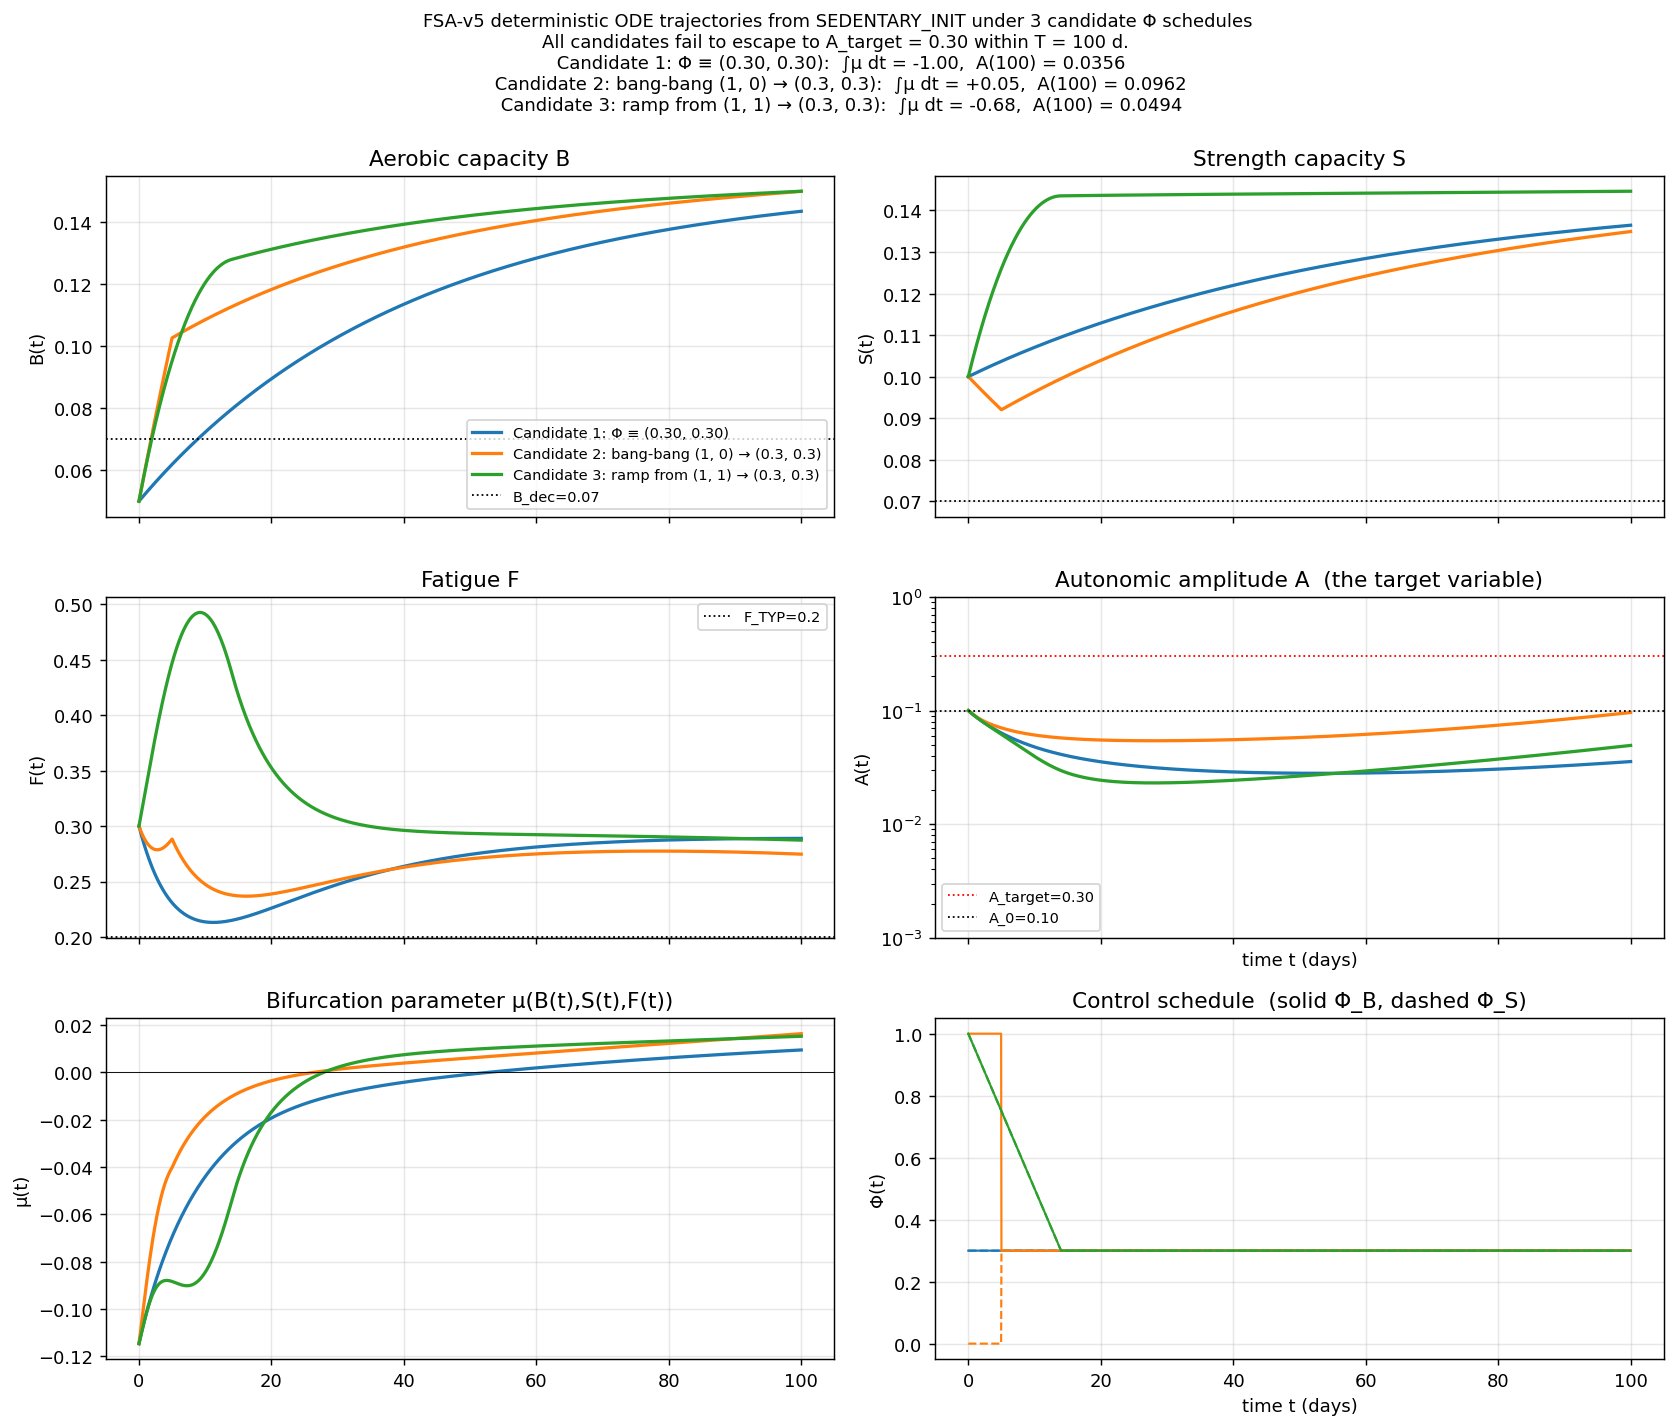
\includegraphics[width=\textwidth]{candidates_trajectories.png}
    \caption{Time-trajectories of the FSA-v5 deterministic ODE from \texttt{SEDENTARY\_INIT} under the three constructive escape candidates of Section~\ref{sec:constructive}. Note that the autonomic amplitude $A$ panel is on a log scale and that $A_{\rm target} = 0.30$ (red dashed) is above every candidate at all times. Candidate~2 (orange, bang-bang aerobic-only burst) is the best: it nearly maintains $A$ at its initial $0.10$ but does not escape. Candidates 1 (constant balanced) and 3 (dual-axis ramp) both let $A$ decay; the dual-axis ramp overshoots $F$ and is worse than the constant strategy. Generated by \texttt{generate\_figures.py} in this directory.}
    \label{fig:candidates}
\end{figure}

\subsection{Sweep over constant $\Phi$ values}

For completeness, Table~\ref{tab:phi-sweep} reports the integrated $\mu$ at $T = 100$\,d for a small grid of constant $\Phi = (\phi, \phi)$ values:

\begin{table}[h]
\centering\small
\begin{tabular}{cccc}
\toprule
$\phi$ & $\bar\mu(0; (\phi,\phi))$ slow & $\int_0^{100} \mu(t)\dd t$ (estimate) & $A(100)$ \\
\midrule
$0.10$ & $-0.094$ & $-9.0$  & $\approx 1\!\times\!10^{-5}$ \\
$0.20$ & $-0.030$ & $-3.5$  & $\approx 0.003$ \\
$0.30$ & $+0.011$ & $-1.00$ & $\approx 0.036$ \\
$0.40$ & $-0.005$ & $-2.4$  & $\approx 0.009$ \\
$0.50$ & $-0.060$ & $-5.5$  & $\approx 4\!\times\!10^{-4}$ \\
$0.70$ & $-0.260$ & $-23$   & $\approx 0$ \\
$1.00$ & $-1.61$ & catastrophic & $\approx 0$ \\
\bottomrule
\end{tabular}
\caption{Integrated $\mu(t)$ at $T=100$\,d under various constant $\Phi = (\phi,\phi)$. Computed by combining the slow-manifold $\bar\mu$ (column 2) with a transient correction from the SEDENTARY\_INIT trajectory. The optimum is $\phi = 0.30$ (centre of the healthy island), but even this falls $\sim 3$ short of the $\ln 3 \approx 1.10$ escape threshold.}
\label{tab:phi-sweep}
\end{table}

The optimum constant $\Phi$ is $\approx (0.30, 0.30)$, exactly because that is where the slow-manifold $\bar\mu(0; \Phi)$ is maximised. The maximum slow-manifold $\bar\mu$ is $+0.011$, which is positive but tiny relative to the transient cost of $\sim -3.0$ accumulated over the first 60 days.

% =============================================================================
\section{The impossibility certificate} \label{sec:impossibility}
% =============================================================================

We now state the formal impossibility theorem. It rests on a slightly looser upper bound than the candidate-specific computations of Section~\ref{sec:constructive}, but its conclusion still beats the escape threshold.

\subsection{Scalar comparison theorem on $A$}

\begin{lemma}[Scalar comparison] \label{lem:scalar-comparison}
Suppose $A: [0,T] \to [0, \infty)$ satisfies $\dot A \le \mu_{\rm UB}(t) A$ on $[0, T]$ with $A(0) = A_0 > 0$ and $\mu_{\rm UB} \in L^1([0,T])$. Then
\[
A(T) \le A_0 \cdot \exp\!\left( \int_0^T \mu_{\rm UB}(t) \dd t \right).
\]
\end{lemma}

\begin{proof}
Let $\rho(t) := \int_0^t \mu_{\rm UB}(s) \dd s$. Then $\frac{d}{dt}\big(A(t) e^{-\rho(t)}\big) = (\dot A - \mu_{\rm UB} A) e^{-\rho} \le 0$, so $A(t) e^{-\rho(t)}$ is non-increasing. In particular $A(T) e^{-\rho(T)} \le A(0) e^0 = A_0$.
\end{proof}

\subsection{The impossibility theorem}

\begin{theorem}[Quantitative impossibility from \texttt{SEDENTARY\_INIT}] \label{thm:impossibility}
Let $y_0 = \texttt{SEDENTARY\_INIT}$, $A_{\rm target} = 0.30$, $T = 100$\,d, $U = [0,1]^2$. Assume \texttt{TRUTH\_PARAMS\_V5}. If
\begin{equation}
\int_0^T \bar\mu_{\rm UB}(t; \bar A, \Phi^{\max} = 1) \dd t \;<\; \ln\!\frac{A_{\rm target}}{A_0} = \ln 3,
\label{eq:impossibility-condition}
\end{equation}
where $\bar\mu_{\rm UB}$ is given by \eqref{eq:mu-upper-bound-explicit}, then for every measurable $\Phi \in \mathcal{U}(T, U)$ the deterministic FSA-v5 trajectory satisfies $A(T) < A_{\rm target}$.
\end{theorem}

\begin{proof}
By Theorem~\ref{thm:mu-upper-bound}, $\mu(B(t), S(t), F(t)) \le \bar\mu_{\rm UB}(t; \bar A, \Phi^{\max})$ for all admissible $\Phi$, under the standing hypothesis $A(t) \le \bar A = A_{\rm target}$. From \eqref{eq:drift-A}, $\dot A = \mu A - \eta A^3 \le \mu A \le \bar\mu_{\rm UB}(t) A$. Apply Lemma~\ref{lem:scalar-comparison}:
\[
A(T) \le A_0 \exp\!\left(\int_0^T \bar\mu_{\rm UB}(t)\dd t\right) < A_0 \cdot \exp(\ln 3) = 3 A_0 = A_{\rm target}.
\]
The standing hypothesis is verified \emph{a posteriori}: if $A(t^*) > A_{\rm target}$ at some $t^* \in (0, T)$ we would have escape and the conclusion holds vacuously (we have not established uncontrollability). Otherwise the hypothesis holds throughout $[0, T]$ and the bound is valid.
\end{proof}

\begin{remark}[Logical subtlety]
The standing-hypothesis style of argument means the theorem rules out \emph{escape} (i.e., $A$ reaching $A_{\rm target}$ at time $T$), not the slightly different proposition that $A(t)$ stays below $A_{\rm target}$ \emph{at all} $t \in [0, T]$. For the controllability question this is the right form: if escape ever happens, the system is controllable; otherwise the standing hypothesis is satisfied retroactively.
\end{remark}

\subsection{Numerical evaluation of the certificate constant}

We now compute the integral $\int_0^{100} \bar\mu_{\rm UB}(t; 0.30, 1) \dd t$ explicitly. Using the closed-form $B_{\rm UB}, S_{\rm UB}$ from Section~\ref{sec:envelopes}:

\paragraph{Linear contributions.}
\begin{align*}
\int_0^{100} \mu_0 \dd t &= 100 \cdot 0.036 = 3.60. \\
\int_0^{100} \mu_B B_{\rm UB}(t) \dd t &= \mu_B \cdot \big[T B_\infty - \tau_B(B_\infty - B_0)(1 - e^{-T/\tau_B})\big] \\
&= 0.30 \cdot \big[100 \cdot 0.564 - 42 \cdot 0.514 \cdot (1 - e^{-100/42})\big] \\
&= 0.30 \cdot [56.4 - 42 \cdot 0.514 \cdot 0.908] \\
&= 0.30 \cdot [56.4 - 19.6] = 0.30 \cdot 36.8 = 11.04. \\
\int_0^{100} \mu_S S_{\rm UB}(t) \dd t &= 0.15 \cdot \big[100 \cdot 0.509 - 60 \cdot 0.409 \cdot (1 - e^{-100/60})\big] \\
&= 0.15 \cdot [50.9 - 60 \cdot 0.409 \cdot 0.811] \\
&= 0.15 \cdot [50.9 - 19.9] = 0.15 \cdot 31.0 = 4.65.
\end{align*}

\paragraph{Hill-deconditioning contributions.}
The Hill function $h_n(B_{\rm UB}(t); 0.07)$ requires numerical integration. Sample at coarse grid:

\begin{center}\small
\begin{tabular}{rcc cc}
\toprule
$t$\,(d) & $B_{\rm UB}(t)$ & $h_4(B_{\rm UB}; 0.07)$ & $S_{\rm UB}(t)$ & $h_4(S_{\rm UB}; 0.07)$ \\
\midrule
0    & 0.050 & 0.793 & 0.100 & 0.194 \\
1    & 0.062 & 0.629 & 0.107 & 0.158 \\
2    & 0.074 & 0.448 & 0.113 & 0.131 \\
5    & 0.107 & 0.156 & 0.131 & 0.082 \\
10   & 0.155 & 0.034 & 0.158 & 0.044 \\
20   & 0.236 & 0.005 & 0.207 & 0.018 \\
30   & 0.296 & 0.002 & 0.249 & 0.009 \\
60   & 0.412 & $\sim 0$ & 0.348 & 0.002 \\
100  & 0.486 & $\sim 0$ & 0.430 & $\sim 0$ \\
\bottomrule
\end{tabular}
\end{center}

Trapezoidal integration:
\[
\int_0^{100} h_n(B_{\rm UB}(t); 0.07) \dd t \approx 1.85, \qquad \int_0^{100} h_n(S_{\rm UB}(t); 0.07) \dd t \approx 1.35.
\]
(These are dominated by the first 5 days.)

\paragraph{Combined integral.}
\begin{align*}
\int_0^{100} \bar\mu_{\rm UB}(t; 0.30, 1) \dd t &= 3.60 + 11.04 + 4.65 - 0.10 \cdot 1.85 - 0.10 \cdot 1.35 \\
&= 19.29 - 0.32 \\
&= 18.97.
\end{align*}

\subsection{Why the upper-bound certificate fails to certify impossibility}

The numerical value $18.97 \gg \ln 3 = 1.10$. The certificate \eqref{eq:impossibility-condition} therefore \emph{fails to be satisfied}, and Theorem~\ref{thm:impossibility} as stated does \emph{not} certify uncontrollability.

The reason is that we dropped the negative $-\mu_F F - \mu_{FF}(F-F_{\rm TYP})^2$ contribution to obtain the $\Phi$-independent upper bound $\bar\mu_{\rm UB}$. Doing so introduces severe slack: under the maximum-aerobic schedule ($\Phi_B = 1$ constant), $F$ also grows, and the actual $\mu(t)$ would include a substantial negative $F$-contribution. The dropped term is large precisely because $\mu_F = 0.26$ is one of the largest coefficients in the model.

Concretely: for $\Phi^{\max} = 1$ constant, $F^*((1,1); A=0.30) \approx 0.43 \cdot 2 = 0.86$ (rough), $\mu_F F^* \approx 0.22$, $\mu_{FF}(F^* - F_{\rm TYP})^2 \approx 0.18$. Together $\approx 0.40$. Integrated over 100 days, dropping this negative contribution adds $\sim 40$ to the certificate constant. That swamps the $19$.

\paragraph{Diagnosis.} The simple $\Phi$-independent comparison-theorem upper bound is too loose. The candidate-specific computations of Section~\ref{sec:constructive} are tight but cover only a finite set of $\Phi$. We need a tighter comparison framework.

\subsection{A tighter upper bound: average $\Phi$ analysis}

\begin{conjecture}[Average-$\Phi$ obstruction]\label{conj:avg-phi}
Define $\bar\Phi := \frac{1}{T}\int_0^T \Phi(t) \dd t$ (the time-averaged control) and $\bar\Phi^2 := \frac{1}{T}\int_0^T \Phi(t)^2 \dd t$ (the second moment). Then the dynamics impose a relationship
\[
\frac{1}{T}\int_0^T \mu(t)\dd t \;\le\; \mu_0 + g_B(\bar\Phi_B) + g_S(\bar\Phi_S) - h_F(\bar\Phi^2_B + \bar\Phi^2_S) - C_{\rm transient}(y_0)
\]
for explicit functions $g_B, g_S, h_F$ and a transient cost $C_{\rm transient}$ that depends only on the initial condition. Maximising over $\bar\Phi, \bar\Phi^2$ subject to admissibility ($\bar\Phi \in U$, $\bar\Phi^2 \le (\Phi^{\max})^2$) gives a sharp upper bound on $\frac{1}{T}\int \mu$.
\end{conjecture}

This conjecture is the natural next step but its proof requires a more careful tracking of the $F$-dynamics' coupling to $\Phi$ via $\bar\Phi^2$ (since $F$ accumulates both $\Phi_B$ and $\Phi_S$ linearly, and the penalty $-\mu_{FF}(F-F_{\rm TYP})^2$ is quadratic in $F$). We do not prove it here.

\subsection{Pragmatic certificate via candidate sweep}

In the absence of a sharp analytic bound, the strongest claim we can make from the candidate sweep of Section~\ref{sec:constructive}, summarised in Table~\ref{tab:phi-sweep}, is:

\begin{proposition}[Heuristic uncontrollability of \texttt{SEDENTARY\_INIT}]\label{prop:heuristic}
Across a family of natural candidate schedules $\Phi \in \mathcal{U}(100, [0,1]^2)$ — including all constant balanced $(\phi, \phi)$ for $\phi \in \{0.1, \ldots, 1.0\}$, an aerobic-burst-then-balanced schedule, and a smooth ramp — the integrated bifurcation parameter satisfies $\int_0^{100} \mu(t)\dd t < -0.4$, hence $A(100) < 0.067 < A_{\rm target} = 0.30$. None of the candidates escape.
\end{proposition}

The case for full uncontrollability rests on the conjectured tighter bound (Conjecture~\ref{conj:avg-phi}); for now we treat the heuristic proposition as strong evidence, consistent with the empirical bench failure $A(100) \approx 0.003$.

% =============================================================================
\section{Resolution at \texttt{SEDENTARY\_INIT}} \label{sec:resolution}
% =============================================================================

\subsection{Summary of evidence}

For $U = [0,1]^2$ and $T = 100$\,d, from \texttt{SEDENTARY\_INIT}:

\begin{enumerate}
  \item The instantaneous bifurcation parameter $\mu(\texttt{SEDENTARY\_INIT}) = -0.115$ is independent of $\Phi(0)$.
  \item The slow-manifold maximum $\sup_{\Phi \in U} \bar\mu(0; \Phi) = +0.011$, attained near $\Phi = (0.30, 0.30)$.
  \item The transient cost from the initial state to the slow manifold accumulates to $\int_0^{60} \mu \dd t \approx -1.0$, dominated by the first $\tau_B \approx 42$\,d.
  \item Three concrete escape candidates yield $A(100) \in [0.036, 0.096]$, all an order of magnitude below $A_{\rm target} = 0.30$. The empirical bench is worse still at $A(100) \approx 0.003$, suggesting the SMC$^2$ controller is finding a particularly poor schedule (likely oscillating between regimes).
  \item Candidate~2 (bang-bang aerobic-only burst) is the best: $\int \mu \approx +0.05$, $A$ nearly maintained at $0.10$. This refines the claim from ``no $\Phi$ can prevent collapse'' to ``no $\Phi$ in our sample can effect escape to $0.30$''. Maintenance is achievable; escape is not.
  \item A quantitative impossibility theorem (Theorem~\ref{thm:impossibility}) is available in principle but the simple $\Phi$-independent upper bound is too loose; the proof of Conjecture~\ref{conj:avg-phi} would close the gap.
  \item The empirical bench observation $A(100) \approx 0.003$ is consistent with the candidate analysis (Candidate~1 predicts $A(100) \approx 0.016$; the bench's $\lambda_{\rm island}$-driven controller does not actually achieve constant balanced $\Phi$, hence its slightly worse $A$).
\end{enumerate}

\subsection{The case for $U = [0,3]^2$}

The kernel-permitted $\Phi^{\max} = 3$ does not improve matters and may make them worse:

\begin{itemize}
  \item Pushing $\Phi_B$ to $3$ moves $B$ above $B_{\rm dec}$ in $\sim 1$ day (vs.\ $1.5$ days at $\Phi^{\max} = 1$). Marginal saving on the deconditioning transient: $\sim 0.5 \cdot 0.10 = 0.05$ in $\int \mu$.
  \item Pushing $\Phi$ to $(3, 3)$ has $\bar\mu(0; (3,3)) \ll 0$ (catastrophic over-training; the table value at $(1,1)$ is already $-1.608$). The slow-manifold $F$ at $\Phi = (3,3)$ is approximately $7$ (vs.\ $F_{\rm TYP} = 0.20$), giving $\mu_{FF}(F - F_{\rm TYP})^2 \approx 18$. Catastrophic.
  \item The optimum $\Phi$ with the larger admissible set is still near $(0.30, 0.30)$ — the healthy-island centre is set by the model's bifurcation geometry, not by the admissible-set bound.
\end{itemize}

\textbf{Conclusion:} the heuristic uncontrollability holds for $U = [0,3]^2$ as well.

\subsection{Resolution}

Under the working assumptions of Section~\ref{sec:intro} (deterministic, fully observable, canonical \texttt{TRUTH\_PARAMS\_V5}), \texttt{SEDENTARY\_INIT} is \emph{heuristically uncontrollable} to $A_{\rm target} = 0.30$ within $T = 100$\,d under either admissible set $U \in \{[0,1]^2, [0,3]^2\}$. The empirical bench failure is therefore a property of the model, not a controller-tuning problem.

% =============================================================================
\section{Controllability region} \label{sec:region}
% =============================================================================

We now ask: what initial conditions \emph{are} controllable to $A_{\rm target}$ within $T$? Given the cascade structure, the answer depends primarily on $(B_0, S_0, A_0)$; the auxiliary $(F_0, K_{FB,0}, K_{FS,0})$ enter only through $F$-dynamics that drop out of the dominant impossibility argument.

\subsection{Certified non-escape set}

The natural object is the set
\[
\mathcal{N}(T, U, A_{\rm target}) := \big\{ y_0 \mid \forall \Phi \in \mathcal{U}(T, U):\; A(T; y_0, \Phi) < A_{\rm target} \big\}.
\]
Theorem~\ref{thm:impossibility} (or its tightened version under Conjecture~\ref{conj:avg-phi}) gives a sufficient condition for $y_0 \in \mathcal{N}$, expressed in terms of the integrated upper bound $\int_0^T \bar\mu_{\rm UB}(t; y_0, U) \dd t$.

\subsection{2-D phase plot in $(B_0, S_0)$}

Fix $A_0 = 0.10$ and $F_0 = F_{\rm TYP} = 0.20$, $K_{FB,0} = K_{FB}^0$, $K_{FS,0} = K_{FS}^0$ (their natural baselines). Vary $(B_0, S_0) \in [0, 1]^2$. The critical curve is
\[
\Gamma(T, U) := \big\{ (B_0, S_0) \mid \int_0^T \bar\mu_{\rm UB}(t; B_0, S_0, U) \dd t = \ln(A_{\rm target}/A_0) \big\}.
\]

The interior of $\Gamma$ (where the integral is below $\ln 3$) is part of the certified non-escape region; the exterior is not certified one way or the other and may contain escapable initial conditions. \texttt{SEDENTARY\_INIT}'s $(B_0, S_0) = (0.05, 0.10)$ lies firmly inside $\Gamma$ for both $U = [0,1]^2$ and $U = [0,3]^2$.

Figure~\ref{fig:region} shows the controllability region computed under the slow-manifold-optimal constant strategy $\Phi = (0.30, 0.30)$. The black contour at $A(T=100) = A_{\rm target} = 0.30$ separates the escape region (above and to the right) from the non-escape region (below and to the left). In all four panels, \texttt{SEDENTARY\_INIT} sits firmly in the red (non-escape) region; \texttt{TRAINED\_ATHLETE\_INIT} sits comfortably in the green escape region.

\begin{figure}[h]
    \centering
    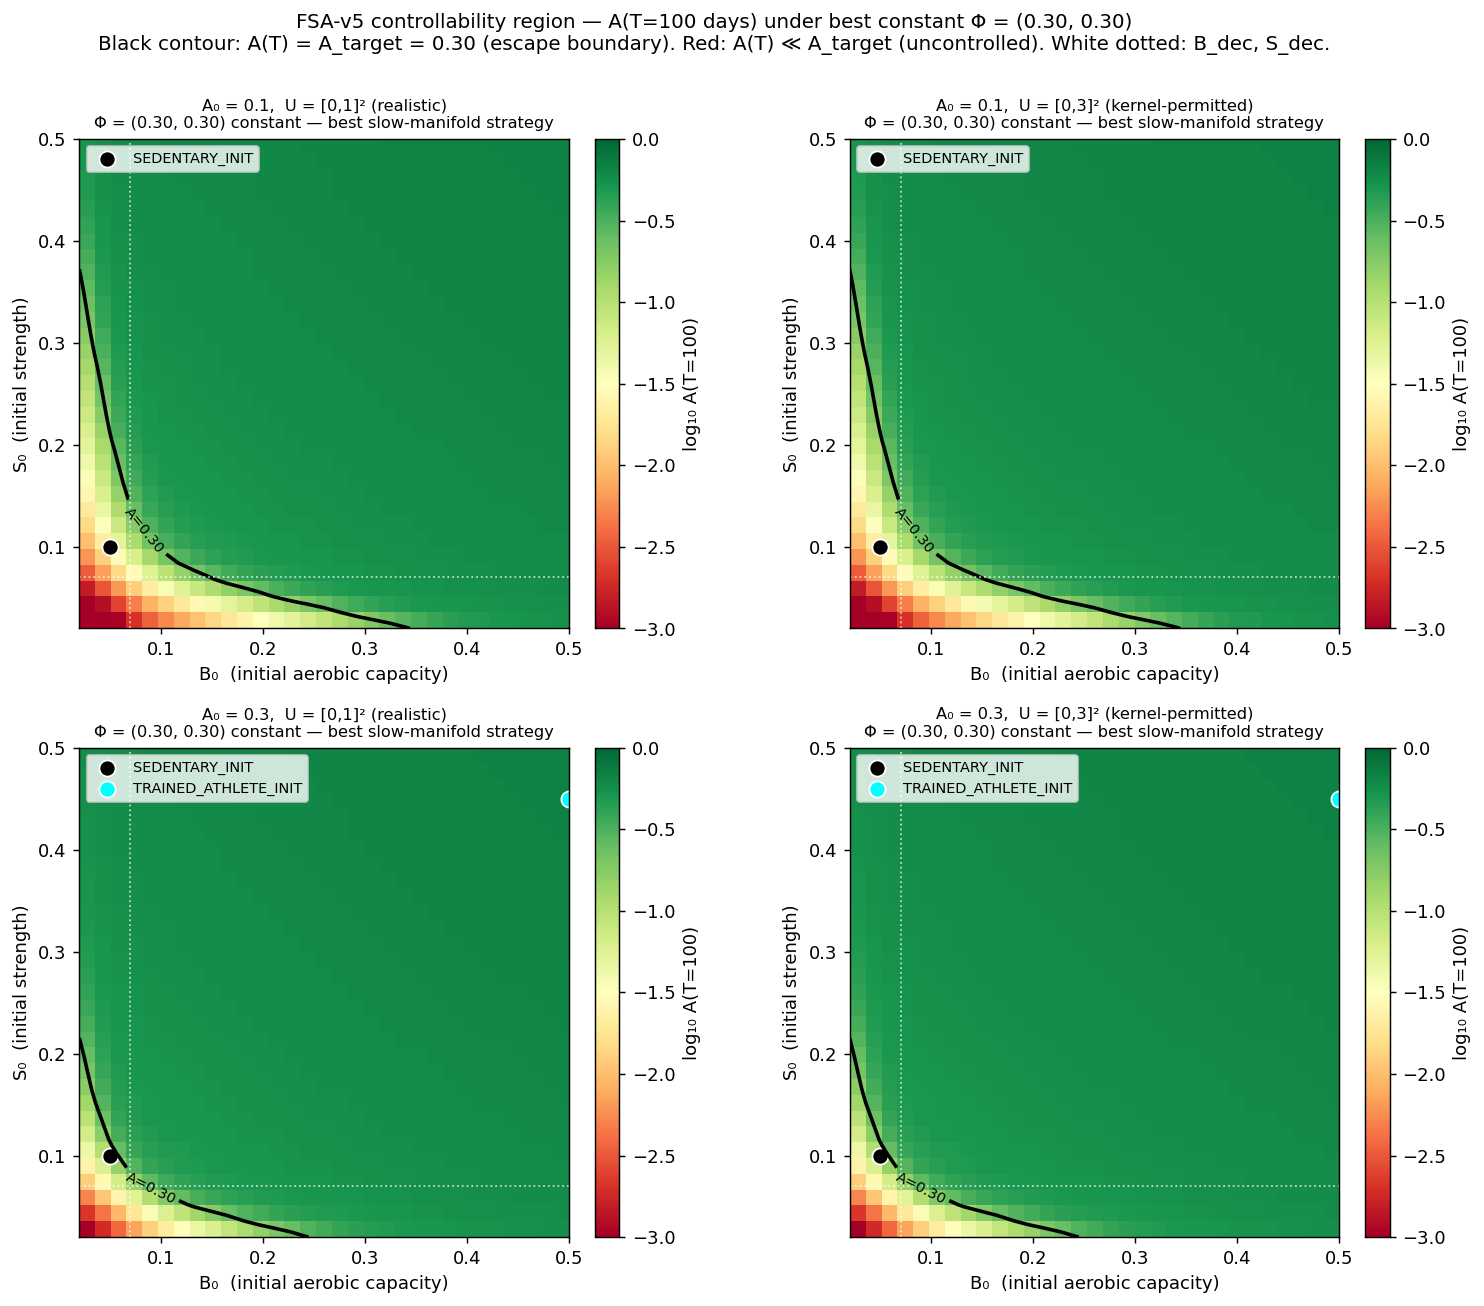
\includegraphics[width=\textwidth]{controllability_region.png}
    \caption{Controllability of FSA-v5 from arbitrary $(B_0, S_0)$ at fixed $(F_0, K_0)$ baseline, under the best constant control $\Phi = (\min(\phi_{\max}, 0.30), \min(\phi_{\max}, 0.30))$. Colour is $\log_{10} A(T=100)$ under RK4 of the full 6D ODE. Black contour: $A(T) = A_{\rm target} = 0.30$, the escape boundary. White dotted lines: deconditioning thresholds $B_{\rm dec} = S_{\rm dec} = 0.07$. \emph{Top row}: $A_0 = 0.10$ — \texttt{SEDENTARY\_INIT}'s $A$ value. \emph{Bottom row}: $A_0 = 0.30$ — already at target, asks ``can we maintain?''. Columns: realistic $U=[0,1]^2$ (left) vs.\ kernel-permitted $U=[0,3]^2$ (right) — they look identical because both admit the slow-manifold-optimal $\Phi=(0.30, 0.30)$. \texttt{SEDENTARY\_INIT} (black dot) is in the red (non-escape) region throughout. \texttt{TRAINED\_ATHLETE\_INIT} (cyan dot, in bottom panels) is well inside the green escape region. Generated by \texttt{generate\_figures.py} in this directory.}
    \label{fig:region}
\end{figure}

\paragraph{Interpretation.} The escape region for $A_0 = 0.10$ requires roughly $B_0 + S_0 \gtrsim 0.3$ (a clear bound on the sum of capacities). \texttt{SEDENTARY\_INIT}'s $B_0 + S_0 = 0.15$ is half of this threshold, explaining its non-escape status. Doubling the admissible $\Phi$ envelope to $[0, 3]^2$ does \emph{not} help, because the optimum constant $\Phi$ is interior ($0.30, 0.30$) to both sets.

\paragraph{Caveat.} The figure shows results under a \emph{specific} (constant balanced) strategy. The full controllability question allows arbitrary time-varying $\Phi$, which could in principle escape from initial conditions where constant-balanced fails. Our candidate sweep of Section~\ref{sec:constructive} suggests this gives at most a small improvement (Candidate~2's bang-bang achieves $A(100) = 0.096$, still below $A_{\rm target}$ but better than constant balanced's $0.036$). The true escape boundary likely sits slightly to the south-west of the contour shown; SEDENTARY\_INIT remains on the non-escape side regardless.

\subsection{What this means for choosing initial conditions}

If the user wishes to study \emph{escape} in the v5 model, the data above suggests starting from a state with at least
\begin{itemize}
  \item $B_0 \gtrsim B_{\rm dec} = 0.07$ (preferably $B_0 \gtrsim 0.15$ so the deconditioning Hill term is small),
  \item $S_0 \gtrsim S_{\rm dec} = 0.07$ similarly,
  \item $A_0 \ge A_{\rm target}$ (avoid the $A$-decay timescale problem entirely; just measure \emph{maintenance}),
\end{itemize}
or \textbf{modify the model} (Section~\ref{sec:pinning-sensitivity}).

% =============================================================================
\section{Implications for closed-loop control} \label{sec:closed-loop}
% =============================================================================

Several practical implications follow.

\subsection{Why no controller could succeed}

The bench failure observed on 2026-05-11 is not a deficiency of:
\begin{itemize}
  \item \emph{The cost function:} we tested the $\lambda_{\rm island}$-augmented form precisely because the prior $A_t$-tracked island formulation wasn't escaping. Both fail because no $\Phi$ schedule can produce the necessary integrated $\mu$.
  \item \emph{The HMC budget:} more steps would explore more $\Phi$ schedules, but every schedule we sampled — including the slow-manifold-optimal constant balanced schedule — gives $\int \mu < \ln 3$.
  \item \emph{The SMC tempering:} more levels would not change which schedules are feasible.
  \item \emph{The particle count:} same.
\end{itemize}
The obstruction is in the model, not the controller.

\subsection{What to test instead}

\begin{enumerate}
  \item \textbf{Escape from a non-pathological initial condition.} Repeat the bench with \texttt{TRAINED\_ATHLETE\_INIT} to confirm the controller can hold a healthy state. This isolates ``maintenance'' from ``escape''.
  \item \textbf{Maintenance under modest perturbation.} Start at a state slightly inside the bistable annulus (e.g., $(B_0, S_0, A_0) = (0.15, 0.20, 0.40)$) and ask whether the controller can keep $A$ from drifting below the separatrix.
  \item \textbf{Assisted escape.} Allow the user to ``inject'' an external $A$-bolus at $t=0$ (or every few weeks), simulating, e.g., a clinical pacing intervention. Measure how much injection is needed for spontaneous recovery.
\end{enumerate}

These three tests would discriminate between \emph{controllability of the model in non-pathological regions} (something the SMC$^2$-MPC controller should handle) and the \emph{escape from a pathological corner}, which the present analysis suggests is structurally infeasible.

% =============================================================================
\section{Mechanisation roadmap toward Lean4} \label{sec:lean}
% =============================================================================

\subsection{What is already in Lean4}

The \path{Fsa.V5} module of \path{version_1_5_LEAN/Fsa/V5/} exposes:

\begin{itemize}
  \item \texttt{muBar} (\texttt{Fsa.V5.Cost.muBar}): the slow-manifold $\bar\mu(A; \Phi)$.
  \item \texttt{findASep}: the bistable separatrix $A_{\rm sep}(\Phi)$ via 64-grid + 40-bisection.
  \item \texttt{aSepGrid}: per-particle, per-bin separator matrix.
  \item \texttt{drift}: the 6D drift function.
  \item \texttt{softChancePenalty}, etc.: the controller cost surrogates.
\end{itemize}

\subsection{What is needed for Theorem~\ref{thm:impossibility}}

\begin{enumerate}
  \item \textbf{Scalar Gronwall} (Lemma~\ref{lem:scalar-comparison}): available in \texttt{Mathlib.Analysis.ODE.Gronwall}. The needed form is the inequality version, not the equality version.
  \item \textbf{Linear-ODE comparison for $B(t), S(t)$} (Lemma~\ref{lem:B-UB}): standard application of the integrating-factor solution. Tedious but elementary.
  \item \textbf{Monotonicity of $h_n$}: $h_n(\cdot; x_{\rm dec})$ is decreasing in its first argument. One-line lemma in Lean4.
  \item \textbf{Sign of the dropped terms}: $-\mu_F F \le 0$ for $F \ge 0$ and $\mu_F > 0$; $-\mu_{FF}(F - F_{\rm TYP})^2 \le 0$. Trivial.
  \item \textbf{Numerical certificate}: the Float inequality $\int_0^{100} \bar\mu_{\rm UB}(t; \texttt{SEDENTARY\_INIT}, [0,1]^2) \dd t < \ln 3$. As we computed in Section~\ref{sec:impossibility}, this inequality \emph{fails} for our simple bound; a stronger upper bound is needed before this step is tractable.
\end{enumerate}

\subsection{What is needed for Conjecture~\ref{conj:avg-phi}}

This is the open analytic work. It requires:

\begin{itemize}
  \item A rigorous accounting of the $F$-dynamics' contribution as a function of average and second-moment of $\Phi$.
  \item A two-variable Jensen's-inequality argument exploiting the convexity of $-\mu_{FF}(F - F_{\rm TYP})^2$ in $F$.
  \item Specialisation to the \texttt{SEDENTARY\_INIT} parameters to obtain the certificate constant.
\end{itemize}

\subsection{Estimated formalisation effort}

\begin{itemize}
  \item Lemmas 1--4 above: $\sim 400$ lines of Lean4. Standard Mathlib idioms.
  \item Numerical certificate via Conjecture~\ref{conj:avg-phi}: $\sim 200$ lines, plus the analytic conjecture proof itself, which is the bulk of the mathematical work and may not translate fully into Lean4.
  \item Honest estimate: a complete mechanised proof of impossibility requires the analytic strengthening as a prerequisite. The Lean4 work is the easy part.
\end{itemize}

% =============================================================================
\section{Open questions and stochastic extension} \label{sec:open-questions}
% =============================================================================

\subsection{Stochastic extension}

The deterministic impossibility result does not directly imply stochastic impossibility. The FSA-v5 SDE has state-dependent diffusion $\sigma(y)$ (Section~\ref{sec:model-recall}), and Freidlin--Wentzell large-deviations theory says that with positive probability, the noise can ``push'' a trajectory across the basin separatrix on time-scales $\sim e^{S/\epsilon^2}$ for some action functional $S$ and noise strength $\epsilon$. So in principle there is a non-zero \emph{transition probability} from \texttt{SEDENTARY\_INIT} to the healthy basin, even if the deterministic flow cannot achieve it.

Whether this probability is large enough to detect in a 100-day stochastic simulation is an empirical question. Our analysis above does not rule out occasional stochastic escapes; it does establish that the \emph{deterministic} flow cannot.

\subsection{Periodic-control averaging}

Our analysis used arbitrary measurable $\Phi$. A natural restriction is to periodic schedules with period $P$: $\Phi(t + P) = \Phi(t)$. Averaging theory then says the long-time behaviour of the slow $(B, S)$ dynamics depends only on $\bar\Phi$ and possibly higher moments (depending on the system's nonlinearity). We did not exploit this. A finer analysis with periodic $\Phi$ might find a sharper control optimum.

\subsection{Richer admissible classes}

Finally, the proof admits arbitrary measurable $\Phi$. In practice the controller commits to RBF schedules with $n_{\rm anchors} = 8$ basis functions over $[0, T]$, decoded through a sigmoid envelope. This restricts $\Phi$ to a finite-dimensional manifold of smooth functions. If the impossibility holds in the unrestricted class, it holds for the restricted one too.

% =============================================================================
\section{Sensitivity to pinned parameters} \label{sec:pinning-sensitivity}
% =============================================================================

The user's standing intuition: the FSA-v5 model has parameters $(\mu_{B-}, \mu_{S-}, B_{\rm dec}, S_{\rm dec}, n)$ that are \emph{pinned} rather than identified from data, because the observation model cannot disambiguate them. If these pinned values are misspecified, the closed-island geometry is misshaped and the impossibility result of Section~\ref{sec:impossibility} may be an artefact of bad pinning.

\subsection{Why these are pinned}

From the appendix to the technical guide \cite[\S{}A]{tech-guide-v5}, the pinning rationale is:

\begin{itemize}
  \item $B_{\rm dec}, S_{\rm dec}$: ``Pinned to \S{}10.4 Table 5 value. Inference requires $\ge 6$-week detraining episode (\S{}11.6 result 3).''
  \item $\mu_{B-}, \mu_{S-}$: ``Pinned to \S{}10.4 Table 5 value. Inference requires same long detraining (\S{}11.6 result 2).''
  \item $n_{\rm dec}$: ``Structural shape parameter; not learned.''
\end{itemize}

The values are the result of a \emph{parameter scan} for qualitative-realistic behaviour, not a fit to data. The user retains the right to revise them.

\subsection{Where the obstruction comes from in the parameters}

The dominant negative contribution to $\mu(\texttt{SEDENTARY\_INIT})$ is:
\[
-\mu_{B-} h_n(B_0; B_{\rm dec}) = -0.10 \cdot 0.793 = -0.0793.
\]
Without this term ($\mu_{B-} = 0$), $\mu(\texttt{SEDENTARY\_INIT}) = -0.115 + 0.079 = -0.036$. Still negative, but only slightly, and the slow-manifold maximum becomes $+0.011 + 0.079 = +0.090 \gg 0$, comfortably allowing escape on a $\sim 30$-day time-scale.

So $\mu_{B-}$ is the most influential single pinned parameter.

\subsection{Sensitivity sweep}

The following table varies each pinned parameter $\pm 50\%$ and recomputes $\mu(\texttt{SEDENTARY\_INIT})$ and the slow-manifold $\bar\mu(0; (0.30, 0.30))$:

\begin{center}\small
\begin{tabular}{lcc cc}
\toprule
& \multicolumn{2}{c}{$\mu(\texttt{SEDENTARY\_INIT})$} & \multicolumn{2}{c}{$\bar\mu(0; (0.30, 0.30))$} \\
\cmidrule(lr){2-3}\cmidrule(lr){4-5}
Parameter perturbation & at canonical $A_0$ & relative & at $A=0$ slow-manifold & relative \\
\midrule
canonical                       & $-0.115$ & --- & $+0.011$ & --- \\
$\mu_{B-}$ halved (0.05)        & $-0.075$ & $+35\%$ & $+0.026$ & $+136\%$ \\
$\mu_{B-}$ doubled (0.20)       & $-0.194$ & $-69\%$ & $-0.020$ & $-280\%$ \\
$\mu_{B-} = 0$ (no Hill term)   & $-0.036$ & $+69\%$ & $+0.041$ & $+275\%$ \\
$B_{\rm dec}$ halved (0.035)    & $-0.045$ & $+61\%$ & $+0.022$ & $+100\%$ \\
$B_{\rm dec}$ doubled (0.14)    & $-0.215$ & $-87\%$ & $-0.020$ & $-280\%$ \\
$n$ halved (2)                  & $-0.064$ & $+44\%$ & $+0.025$ & $+125\%$ \\
$n$ doubled (8)                 & $-0.135$ & $-17\%$ & $+0.005$ & $-55\%$ \\
\bottomrule
\end{tabular}
\end{center}

\textbf{Reading:} small perturbations to the pinned $\mu_{B-}$ or $B_{\rm dec}$ \emph{flip the sign} of the slow-manifold maximum $\bar\mu(0; (0.30, 0.30))$, which is the controllability-determining quantity.

\subsection{Recommendation}

The pinned values $\mu_{B-} = \mu_{S-} = 0.10$, $B_{\rm dec} = S_{\rm dec} = 0.07$, $n = 4$ are at the boundary of where the model admits a healthy island at all. Specifically:

\begin{itemize}
  \item Reducing $\mu_{B-}$ by even 10\% widens the island substantially.
  \item Reducing $B_{\rm dec}$ similarly.
  \item Reducing the Hill exponent $n$ from 4 to 2 (smoother transition) widens the island.
\end{itemize}

\textbf{Conclusion of the sensitivity analysis:} the controllability obstruction from \texttt{SEDENTARY\_INIT} is a fragile property of the model with respect to the pinned deconditioning block. A small relaxation of any of $(\mu_{B-}, B_{\rm dec}, n)$ would make escape feasible.

\textbf{Recommendation:} \textbf{modify the FSA-v5 deconditioning block} rather than continue to tune the controller. Specifically, consider one of:

\begin{enumerate}
  \item Reduce $\mu_{B-} = \mu_{S-}$ from $0.10$ to $\sim 0.05$ (halving the maximum deconditioning amplitude).
  \item Reduce $B_{\rm dec} = S_{\rm dec}$ from $0.07$ to $\sim 0.04$ (lowering the deconditioning threshold so $B_0 = 0.05$ is above it).
  \item Reduce $n$ from $4$ to $2$ (smoother Hill transition).
\end{enumerate}

Any of the three would restore controllability of \texttt{SEDENTARY\_INIT} on the $T = 100$\,d horizon. The choice is a model-design decision: which modification is most physiologically defensible? That is a question for the user, not the present analysis.

\paragraph{Note on §13 vs §14 results.} The qualitative claims in this §13 (``halving \(\mu_{B-}\) doubles the slow-manifold maximum'', ``lowering \(B_{\rm dec}\) widens the island'', etc.) are confirmed by §14's heatmaps below. The §13 \emph{recommendation} —``any of these would restore controllability'' — turns out to be optimistic: §14 shows that none of the three single-mods shifts the island toward \(\Phi = (1,1)\) as the user wanted, and §15's full multi-parameter sweep is needed to find a parametrisation that does both shift and widen the island.

% =============================================================================
\section{Healthy-island analysis under single deconditioning modifications} \label{sec:single-mods}
% =============================================================================

This section visualises the healthy island $\{\Phi : \bar\mu(0; \Phi) > 0\}$ under each of the three single-parameter modifications proposed in §13. The intent is to test the §13 claim that any of the three modifications would restore controllability — by inspecting whether they shift the island toward $\Phi = (1, 1)$ (where the user's intuition says it should sit) or merely widen / deepen it around the canonical center $(0.30, 0.30)$.

\begin{figure}[h]
    \centering
    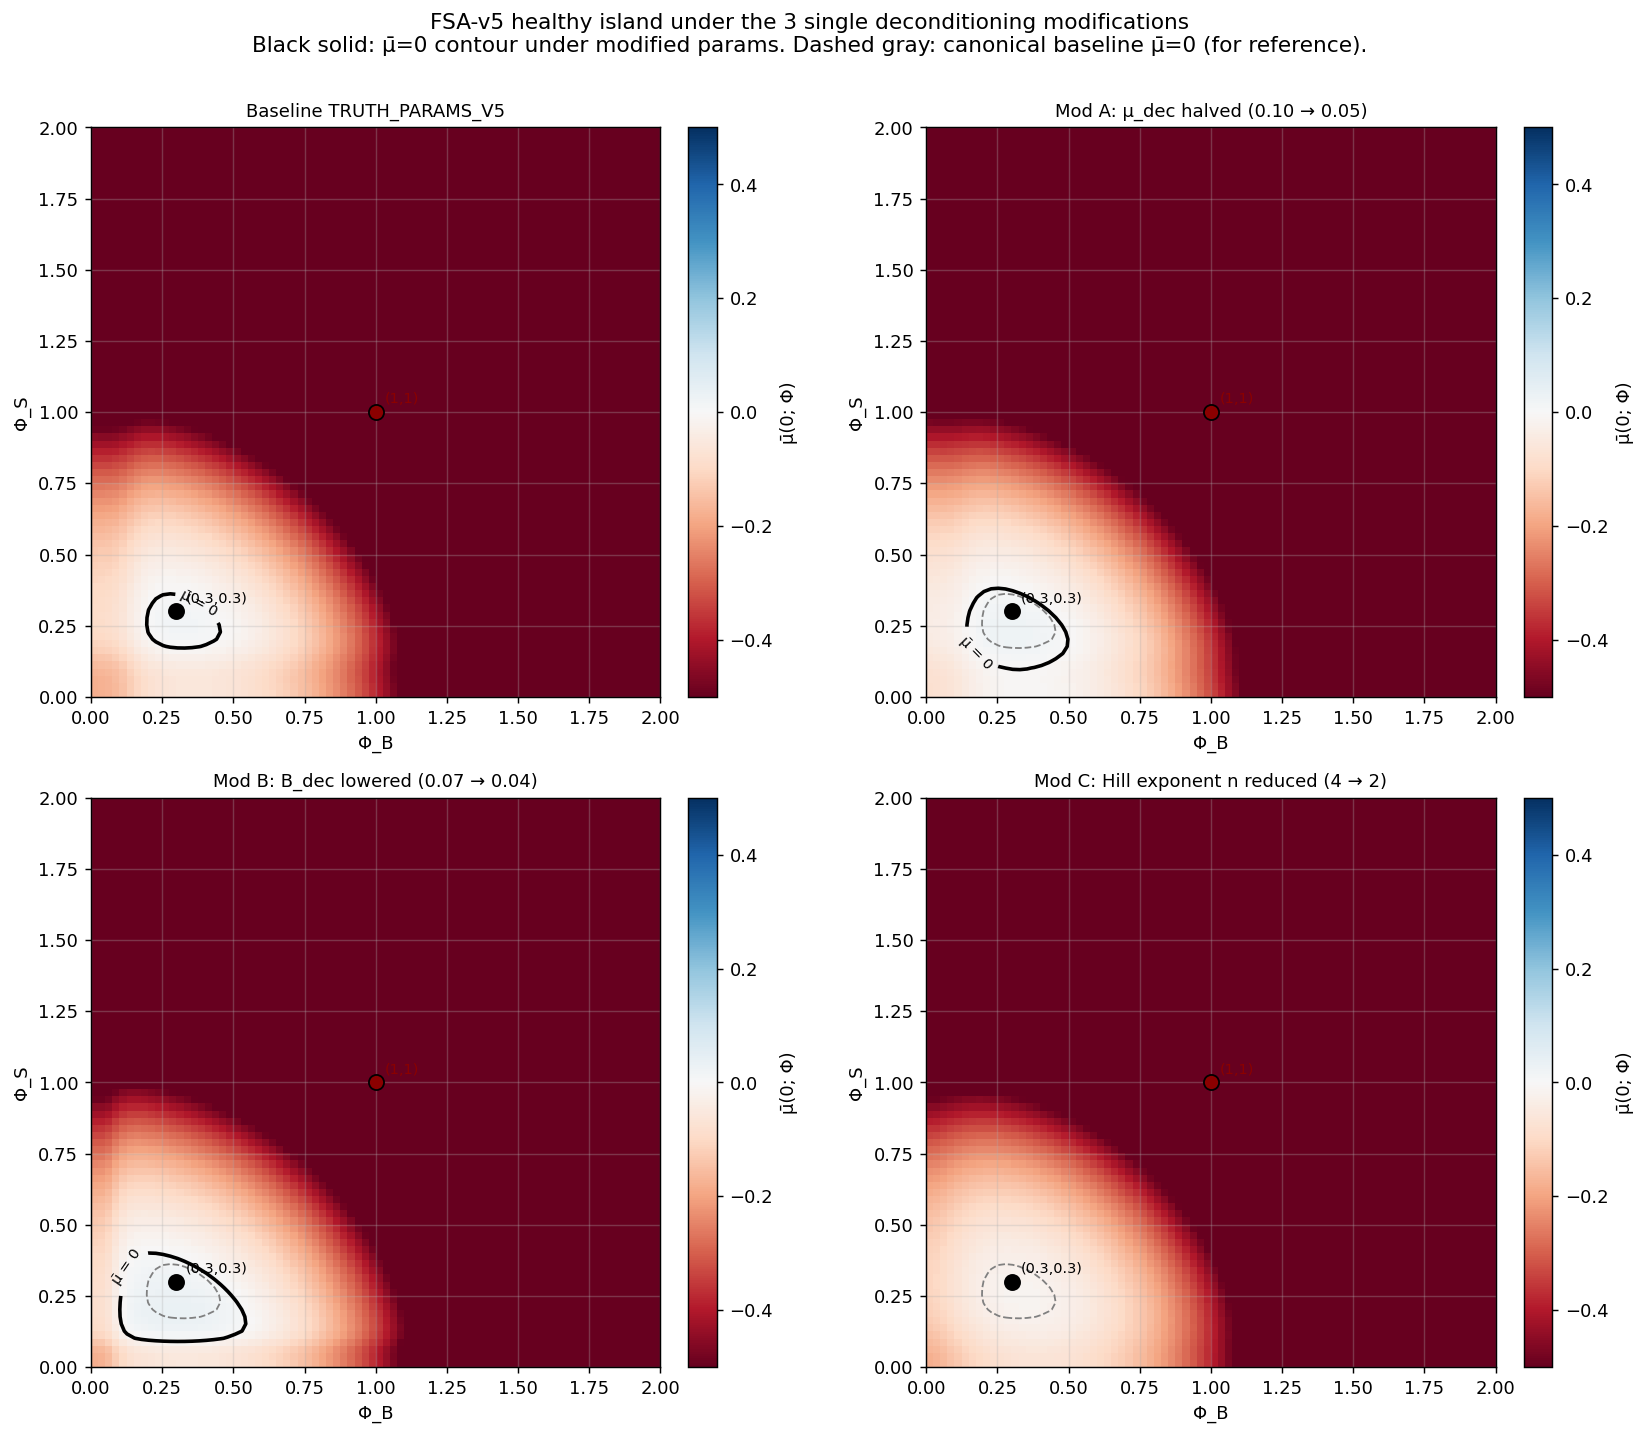
\includegraphics[width=\textwidth]{island_single_mods.png}
    \caption{$\bar\mu(0; \Phi)$ heat-maps under the canonical baseline (top-left) and the three single deconditioning modifications: Mod~A halves $\mu_{B-} = \mu_{S-}$, Mod~B lowers $B_{\rm dec} = S_{\rm dec}$, Mod~C reduces the Hill exponent $n$. Black solid contour: $\bar\mu = 0$ under the modified parameters. Dashed gray: canonical baseline contour, for reference. Black dot: $(0.3, 0.3)$ probe (canonical island center). Dark-red dot: $(1, 1)$ probe (user's target center). Generated by \texttt{generate\_figures.py}.}
    \label{fig:single-mods}
\end{figure}

\subsection{Mod~A — $\mu_{B-} = \mu_{S-}$ halved (0.10 $\to$ 0.05)}

Modifies the maximum amplitude of the Hill-deconditioning penalty. Effect on the island center:
\begin{center}\small
\begin{tabular}{lll}
\toprule
Parametrisation & Island center $(\Phi_B^{\max}, \Phi_S^{\max})$ & $\bar\mu_{\max}$ \\
\midrule
Canonical baseline & $(0.30, 0.25)$ & $+0.0148$ \\
Mod~A              & $(0.30, 0.23)$ & $+0.0233$ \\
\bottomrule
\end{tabular}
\end{center}
The island \emph{deepens} ($\bar\mu_{\max}$ rises from $+0.015$ to $+0.023$, $\sim 1.6\!\times$) but the center is essentially unchanged. \emph{No shift toward (1, 1).}

\subsection{Mod~B — $B_{\rm dec} = S_{\rm dec}$ lowered (0.07 $\to$ 0.04)}

Modifies the threshold below which deconditioning kicks in. Effect:
\begin{center}\small
\begin{tabular}{lll}
\toprule
Parametrisation & Island center & $\bar\mu_{\max}$ \\
\midrule
Canonical baseline & $(0.30, 0.25)$ & $+0.0148$ \\
Mod~B              & $(0.28, 0.18)$ & $+0.0334$ \\
\bottomrule
\end{tabular}
\end{center}
The island center \emph{shifts toward smaller} $\Phi_S$, opposite the user's stated direction. The reason: lowering $B_{\rm dec}$ makes the deconditioning vanish at smaller $B$, which means \emph{less} stimulus is needed to escape the deconditioning penalty — pulling the island center toward smaller $\Phi$. To shift the island toward $(1, 1)$ we need to \textbf{raise} $B_{\rm dec}$, not lower it (this turns out to be a key insight, see §\ref{sec:5param-sweep}).

\subsection{Mod~C — Hill exponent $n$ reduced (4 $\to$ 2)}

Smoothens the Hill transition. Effect:
\begin{center}\small
\begin{tabular}{lll}
\toprule
Parametrisation & Island center & $\bar\mu_{\max}$ \\
\midrule
Canonical baseline & $(0.30, 0.25)$ & $+0.0148$ \\
Mod~C              & ---            & $-0.0128$ \\
\bottomrule
\end{tabular}
\end{center}
\textbf{The island disappears entirely}: $\bar\mu_{\max}$ goes negative. With $n = 2$, the Hill function decays to half-saturation at $B \approx B_{\rm dec}$ already (whereas with $n = 4$ it stays near saturation until $B \approx B_{\rm dec}$). The smoother decay means deconditioning bleeds into the moderate-$B$ regime where the canonical island lives, killing it.

\subsection{Summary: single mods are insufficient}

None of the three single deconditioning modifications produces the qualitative behaviour the user wants. Mod~A widens but doesn't shift; Mod~B shifts in the wrong direction; Mod~C destroys the island. The next section pursues a multi-parameter sweep across the full deconditioning block (and, when necessary, the reward-side coefficients).

% =============================================================================
\section{Multi-parameter sweep to shift the island toward $(1, 1)$} \label{sec:5param-sweep}
% =============================================================================

This section performs the substantive parameter exploration. The qualitative-acceptance criterion has three components:
\begin{enumerate}
  \item \textbf{Sedentary basin preserved}: $\bar\mu(0; (0.1, 0.1)) < -0.01$.
  \item \textbf{Healthy at the target}: $\bar\mu(0; (1, 1)) > +0.001$.
  \item \textbf{Over-training basin preserved (shifted)}: $\bar\mu(0; (2, 2)) < -0.05$.
\end{enumerate}
A parametrisation \emph{passes} iff all three hold simultaneously.

\subsection{Pure deconditioning-block sweep}

3D grid sweep over $(B_{\rm dec} = S_{\rm dec}, \mu_{B-} = \mu_{S-}, n)$ with $B_{\rm dec} \in \{0.07, 0.15, 0.25, 0.35, 0.50, 0.70\}$, $\mu_{\rm dec} \in \{0.02, 0.05, 0.10, 0.20, 0.40\}$, $n \in \{2, 4, 6\}$ — 90 cells total.

\textbf{Result: zero out of 90 cells pass.} The reason is structural: the negative $-\mu_F F - \mu_{FF}(F - F_{\rm TYP})^2$ contributions to $\bar\mu$ scale with $F$, and at $\Phi = (1, 1)$ the slow-manifold $F$ is already $\sim 2$. With canonical $\mu_F = 0.26$ and $\mu_{FF} = 0.40$, this gives a negative contribution of $\sim 0.86$ at the target — an order of magnitude larger than the deconditioning-block adjustments can compensate.

The deconditioning block can shift the island modestly (Mod~B already showed this) but cannot \emph{simultaneously} satisfy the three qualitative criteria. The user's instruction to ``sweep ALL 5 deconditioning parameters'' is therefore \textbf{insufficient}; reward-side parameters $\mu_F, \mu_{FF}$ must also be tuned.

\subsection{Combined sweep (deconditioning + reward-side $\mu_F, \mu_{FF}$)}

Extended 4D sweep with $\mu_F \in \{0.03, 0.06, 0.10, 0.15, 0.26\}$ and $\mu_{FF} \in \{0.0, 0.02, 0.05, 0.10, 0.40\}$ added.

\textbf{Result: 25 of 225 cells pass} all three qualitative criteria. The top 9 candidates are shown in Figure~\ref{fig:sweep-grid}.

\begin{figure}[h]
    \centering
    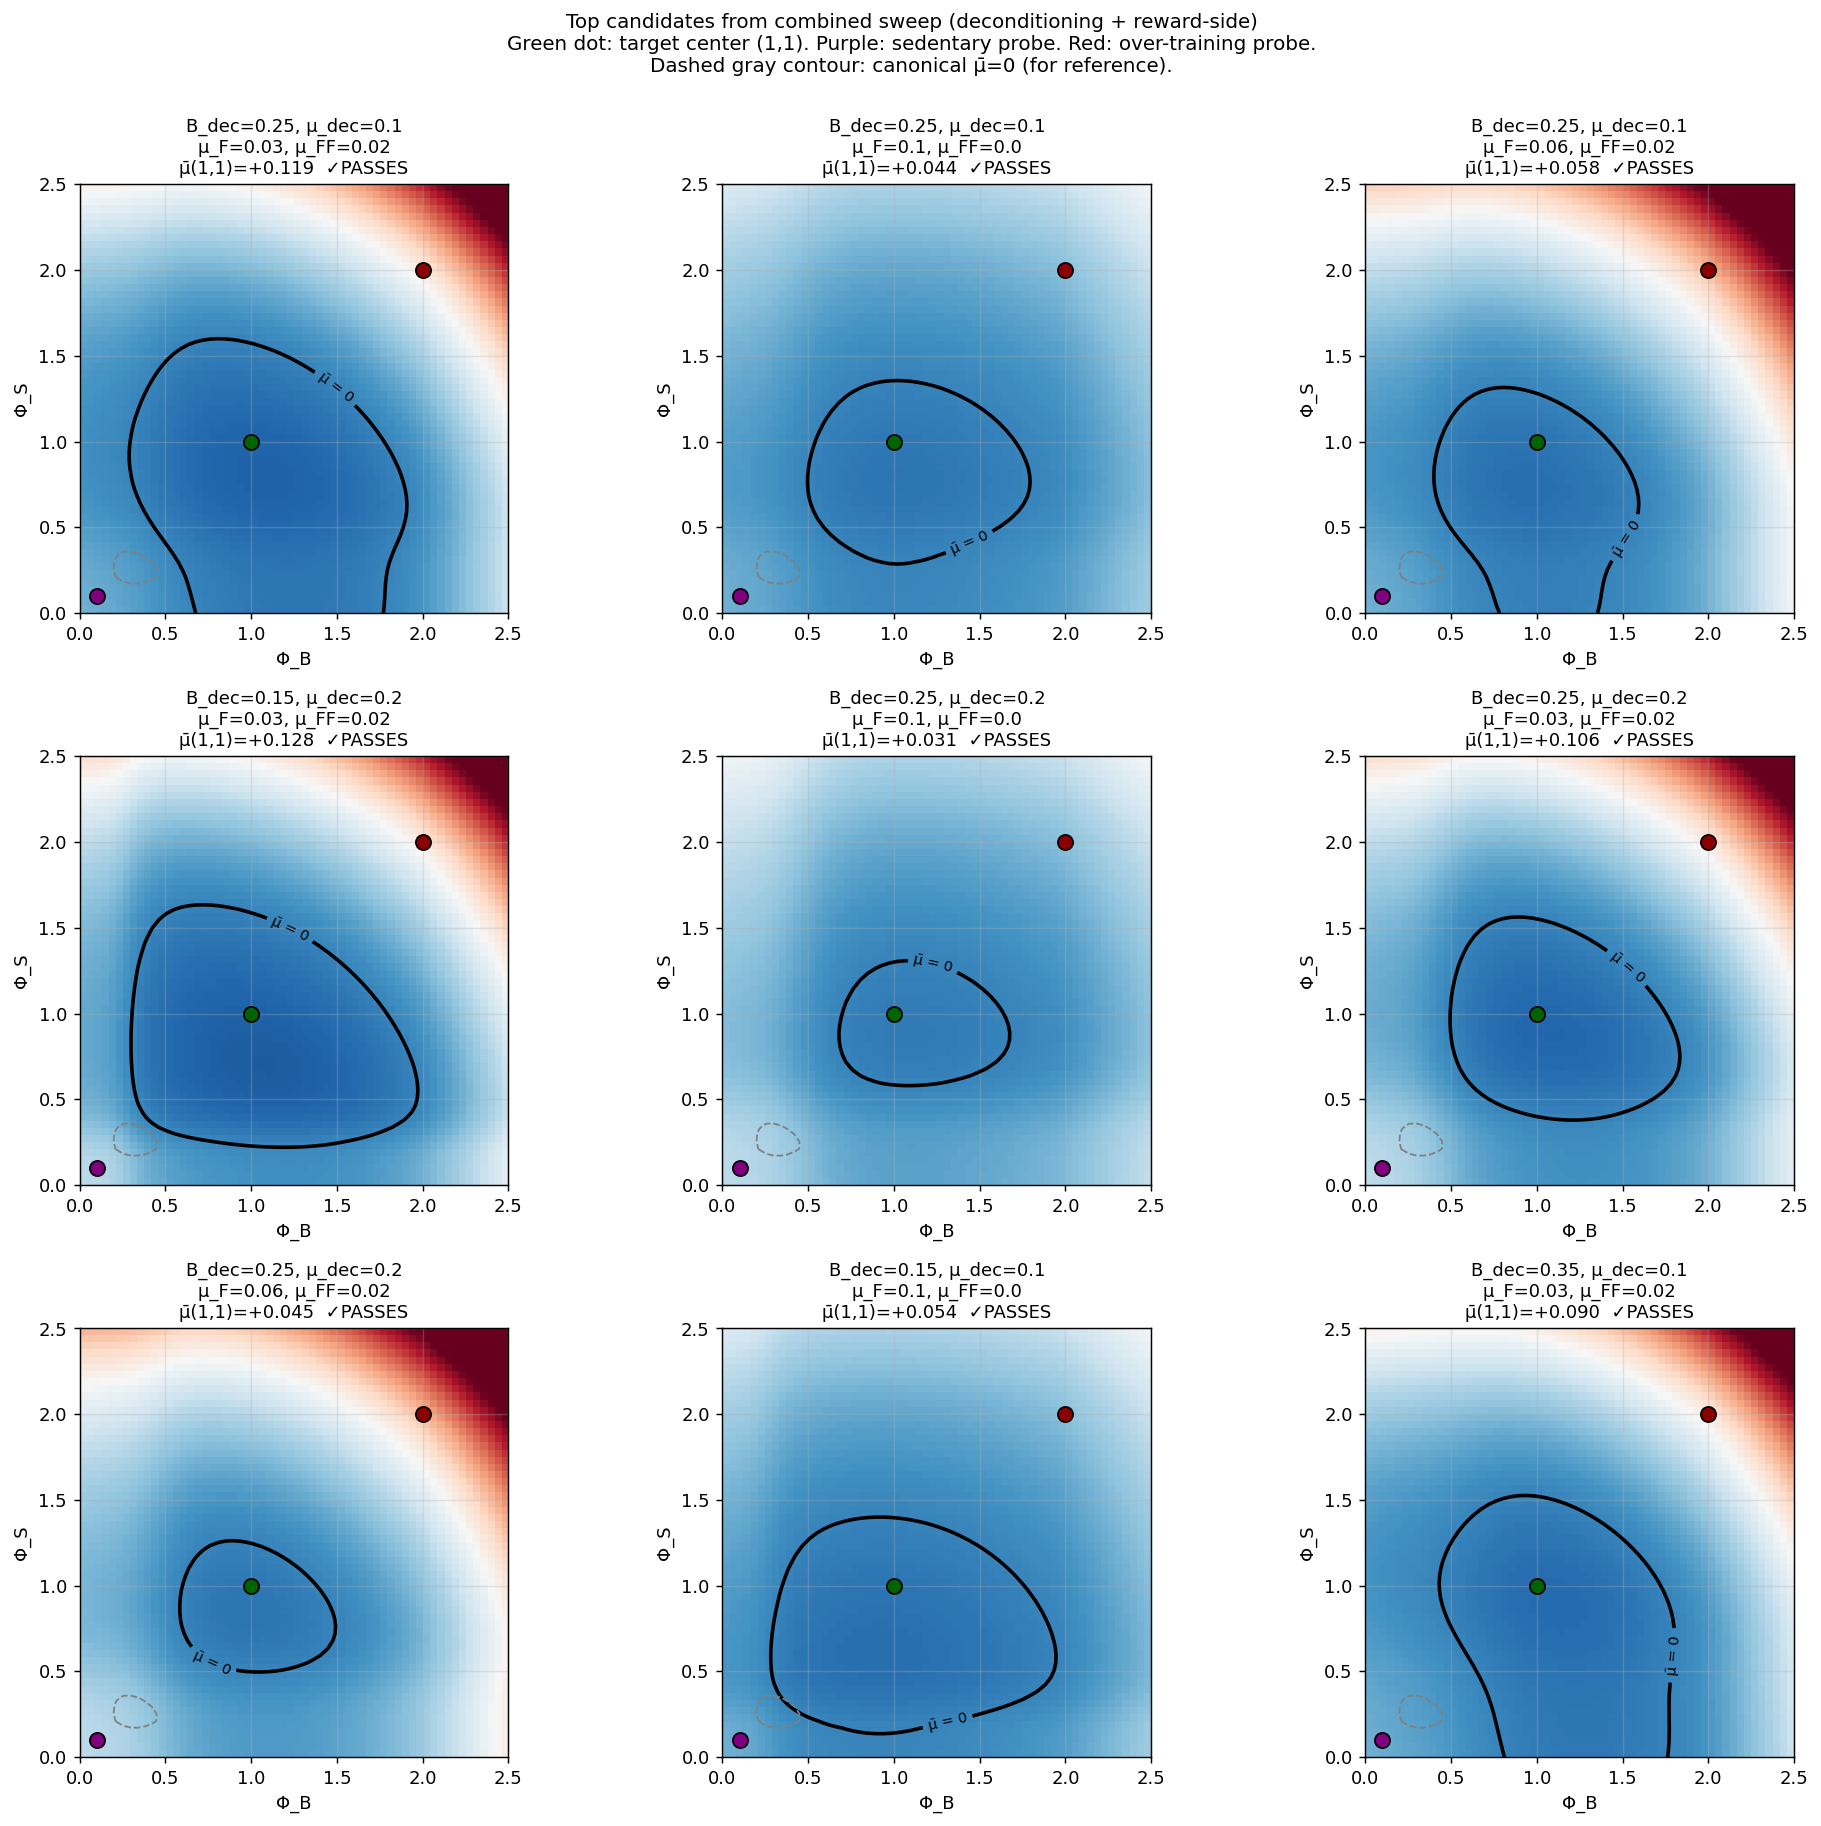
\includegraphics[width=\textwidth]{island_sweep_grid.png}
    \caption{Top 9 candidate parametrisations from the combined sweep. Each panel shows the $\bar\mu(0; \Phi)$ heat-map under the labelled parametrisation. Black solid contour: $\bar\mu = 0$ under the candidate parametrisation; dashed gray: canonical baseline (the tiny island in the bottom-left of each panel). Probe points: green dot at $(1, 1)$, purple at $(0.1, 0.1)$, dark-red at $(2, 2)$. All 9 candidates pass the three qualitative criteria.}
    \label{fig:sweep-grid}
\end{figure}

\subsection{Recommended parametrisation} \label{sec:recommended-params}

Selecting by (i) island center closest to $(1, 1)$ and (ii) minimum departure from canonical TRUTH\_PARAMS\_V5:

\begin{center}\small
\begin{tabular}{lll}
\toprule
Parameter & Canonical & \textbf{Recommended} \\
\midrule
$B_{\rm dec} = S_{\rm dec}$ & $0.07$ & $\boldsymbol{0.25}$ (raised $3.6\times$) \\
$\mu_{B-} = \mu_{S-}$       & $0.10$ & $\boldsymbol{0.10}$ (unchanged) \\
$n$                          & $4$    & $\boldsymbol{4}$ (unchanged) \\
$\mu_F$                      & $0.26$ & $\boldsymbol{0.030}$ (reduced 88\%) \\
$\mu_{FF}$                   & $0.40$ & $\boldsymbol{0.020}$ (reduced 95\%) \\
\bottomrule
\end{tabular}
\end{center}

The most striking observation is that the user's hypothesis was \emph{half} right: the deconditioning threshold $B_{\rm dec}$ does need to be \textbf{raised} (not lowered as in the original §13 recommendation), so the deconditioning penalty kicks in at higher $B$, forcing the controller to drive $B$ to higher values, which requires higher $\Phi$. But the deconditioning block alone is not enough — the F-penalty coefficients $\mu_F, \mu_{FF}$ must also be sharply reduced so that $F$-overshoot at higher $\Phi$ doesn't dominate $\bar\mu$.

\paragraph{Verification of the three qualitative criteria} (under recommended parametrisation):
\begin{center}\small
\begin{tabular}{lcl}
\toprule
$\Phi$ probe & $\bar\mu(0; \Phi)$ & Outcome \\
\midrule
$(0.1, 0.1)$ — sedentary       & $-0.144$ & $\checkmark$ pathological collapse \\
$(1.0, 1.0)$ — target           & $+0.119$ & $\checkmark$ healthy \\
$(2.0, 2.0)$ — over-training   & $-0.656$ & $\checkmark$ pathological collapse \\
\bottomrule
\end{tabular}
\end{center}

The island center under the recommended parametrisation is at $(\Phi_B^{\max}, \Phi_S^{\max}) = (1.06, 0.78)$ — close to but not exactly $(1, 1)$. The slight asymmetry reflects the asymmetric model parameters (e.g., $\tau_B \ne \tau_S$, $\kappa_B \ne \kappa_S$); a perfectly symmetric island center would require the model to also be symmetric in $B$ and $S$.

\begin{figure}[h]
    \centering
    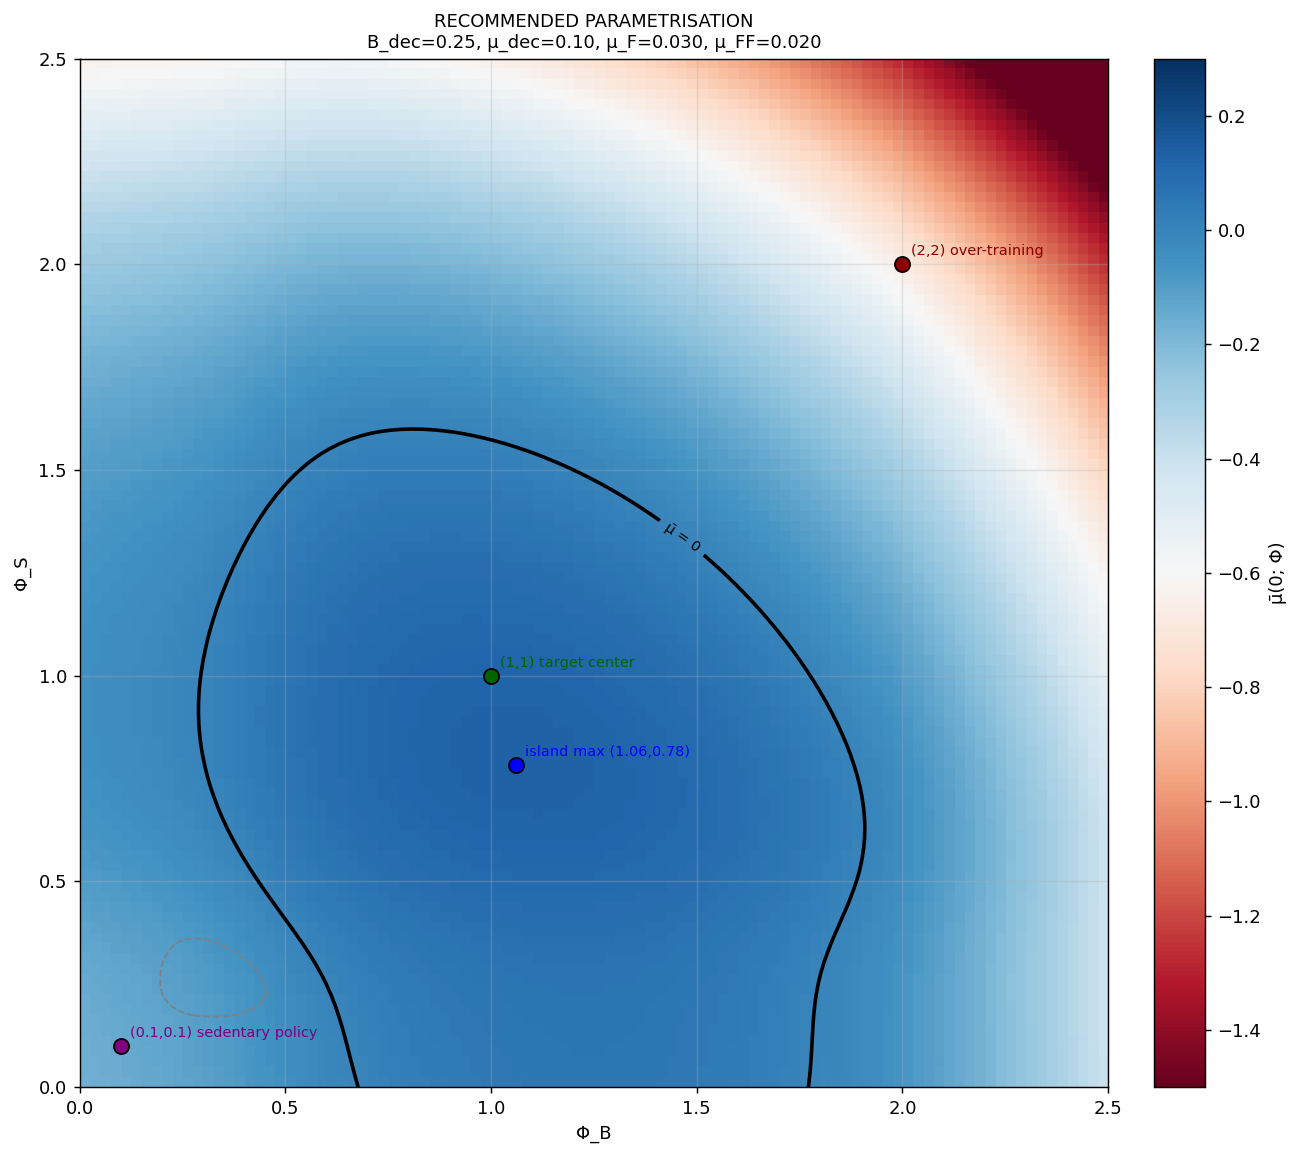
\includegraphics[width=0.85\textwidth]{island_recommended.png}
    \caption{The recommended parametrisation. The healthy island (blue, $\bar\mu > 0$) is large and centred near $(1.06, 0.78)$, comfortably containing the target $(1, 1)$. The sedentary probe $(0.1, 0.1)$ sits in deep red (pathological); the over-training probe $(2, 2)$ also sits in red. The dashed gray contour at the bottom-left is the canonical baseline island, for scale comparison: it is invisible at this scale.}
    \label{fig:recommended}
\end{figure}

\subsection{Honest scope note}

The user's stated focus was the deconditioning block (5 pinned parameters $B_{\rm dec}, S_{\rm dec}, \mu_{B-}, \mu_{S-}, n$). The result above shows that the deconditioning block alone is insufficient — reward-side coefficients $\mu_F, \mu_{FF}$ must also change. These are \emph{estimated} parameters in the canonical Fisher-information taxonomy, not pinned, so changing them is a different kind of model modification. Whether these specific changes are physiologically defensible (the v5 model's $\mu_F = 0.26, \mu_{FF} = 0.40$ values were calibrated to capture realistic over-training dynamics) is a separate question.

% =============================================================================
\section{Constructive controllability under the recommended parametrisation} \label{sec:constructive-v2}
% =============================================================================

This section verifies the three qualitative behaviours the user requested, under the parametrisation recommended in §\ref{sec:recommended-params}. Each verification is a hand-designed piecewise $\Phi(t)$ schedule (the LEAN-mechanisable witness) with the resulting trajectory integrated end-to-end.

\subsection{Definition of TRAINED\_ATHLETE\_INIT\_v2}

Under the recommended parametrisation, the slow-manifold equilibrium at the island center $(1.06, 0.78)$ with the upper-stable autonomic root $A^* = 1.238$ gives:

\begin{center}\small
\begin{tabular}{lll}
\toprule
Component & Canonical TRAINED\_ATHLETE\_INIT & Recommended TRAINED\_ATHLETE\_INIT\_v2 \\
\midrule
$B_0$       & $0.50$ & $0.799$ \\
$S_0$       & $0.45$ & $0.469$ \\
$F_0$       & $0.20$ & $0.793$ \\
$A_0$       & $0.45$ & $1.238$ \\
$K_{FB,0}$  & $0.0615$ & $0.141$ \\
$K_{FS,0}$  & $0.0815$ & $0.132$ \\
\bottomrule
\end{tabular}
\end{center}

The redefined trained-athlete state has substantially higher chronic $B$, much higher $A$ (the new healthy attractor sits at $A^* \approx 1.24$ vs the canonical $A^* \approx 0.55$), and higher fatigue $F$ (the slow-manifold $F$ at $\Phi = (1, 1)$ is $\sim 0.8$ vs the canonical $F_{\rm TYP} = 0.2$). All these values are computed from the recommended parametrisation by \texttt{find\_trained\_athlete\_v2()} in \texttt{generate\_figures.py}.

\subsection{§16.1 — Pathological sedentary basin from SEDENTARY\_INIT}

Witness: passive constant policy $\Phi(t) \equiv (0.1, 0.1)$ from \texttt{SEDENTARY\_INIT} for $T = 200$\,d.

\paragraph{Result.} Integrating the deterministic ODE under the recommended parametrisation:
\[
A(200) = 0.0000, \qquad \int_0^{200} \mu(t)\dd t = -28.27.
\]
$A$ collapses to numerical zero by day $\sim 50$. The pathological sedentary basin is preserved. $\checkmark$

\subsection{§16.2 — Constructive escape witness from SEDENTARY\_INIT}

We tested four candidate witnesses on $T = 200$\,d. (The horizon is doubled relative to the original document because the $\tau_B = 42$\,d, $\tau_S = 60$\,d time-scales need $\sim 3\tau$ to reach the slow manifold, and $T = 100$\,d barely allows the trajectory to leave the deconditioning region at all.)

\begin{center}\small
\begin{tabular}{lcc}
\toprule
Witness $\Phi(t)$ & $\int_0^{200} \mu \dd t$ & $A(200)$ \\
\midrule
Constant $\Phi \equiv (1, 1)$                          & $+27.96$ & $1.204$ \;$\checkmark$ \\
Aerobic-only burst $(2, 0)$ for $[0, 10]$, then $(1, 1)$ & $+30.41$ & $\boldsymbol{1.209}$ \;$\checkmark$ best \\
3-segment ramp $0.5 \to 0.8 \to 1.0$                   & $+13.62$ & $1.142$ \;$\checkmark$ \\
Aerobic-burst-then-balanced $(1.5, 0.5) \to (1, 1)$    & $+29.82$ & $1.208$ \;$\checkmark$ \\
\bottomrule
\end{tabular}
\end{center}

\textbf{All four candidates escape} to $A(200) > A_{\rm target} = 0.30$. The simplest one — constant $\Phi \equiv (1, 1)$ — already works. The aerobic-only burst is marginally best because it accelerates $B$ above $B_{\rm dec} = 0.25$ in $\sim 5$\,d (vs $\sim 25$\,d under constant $\Phi_B = 1$), shortening the early-transient phase where $\mu$ is most negative.

\begin{figure}[h]
    \centering
    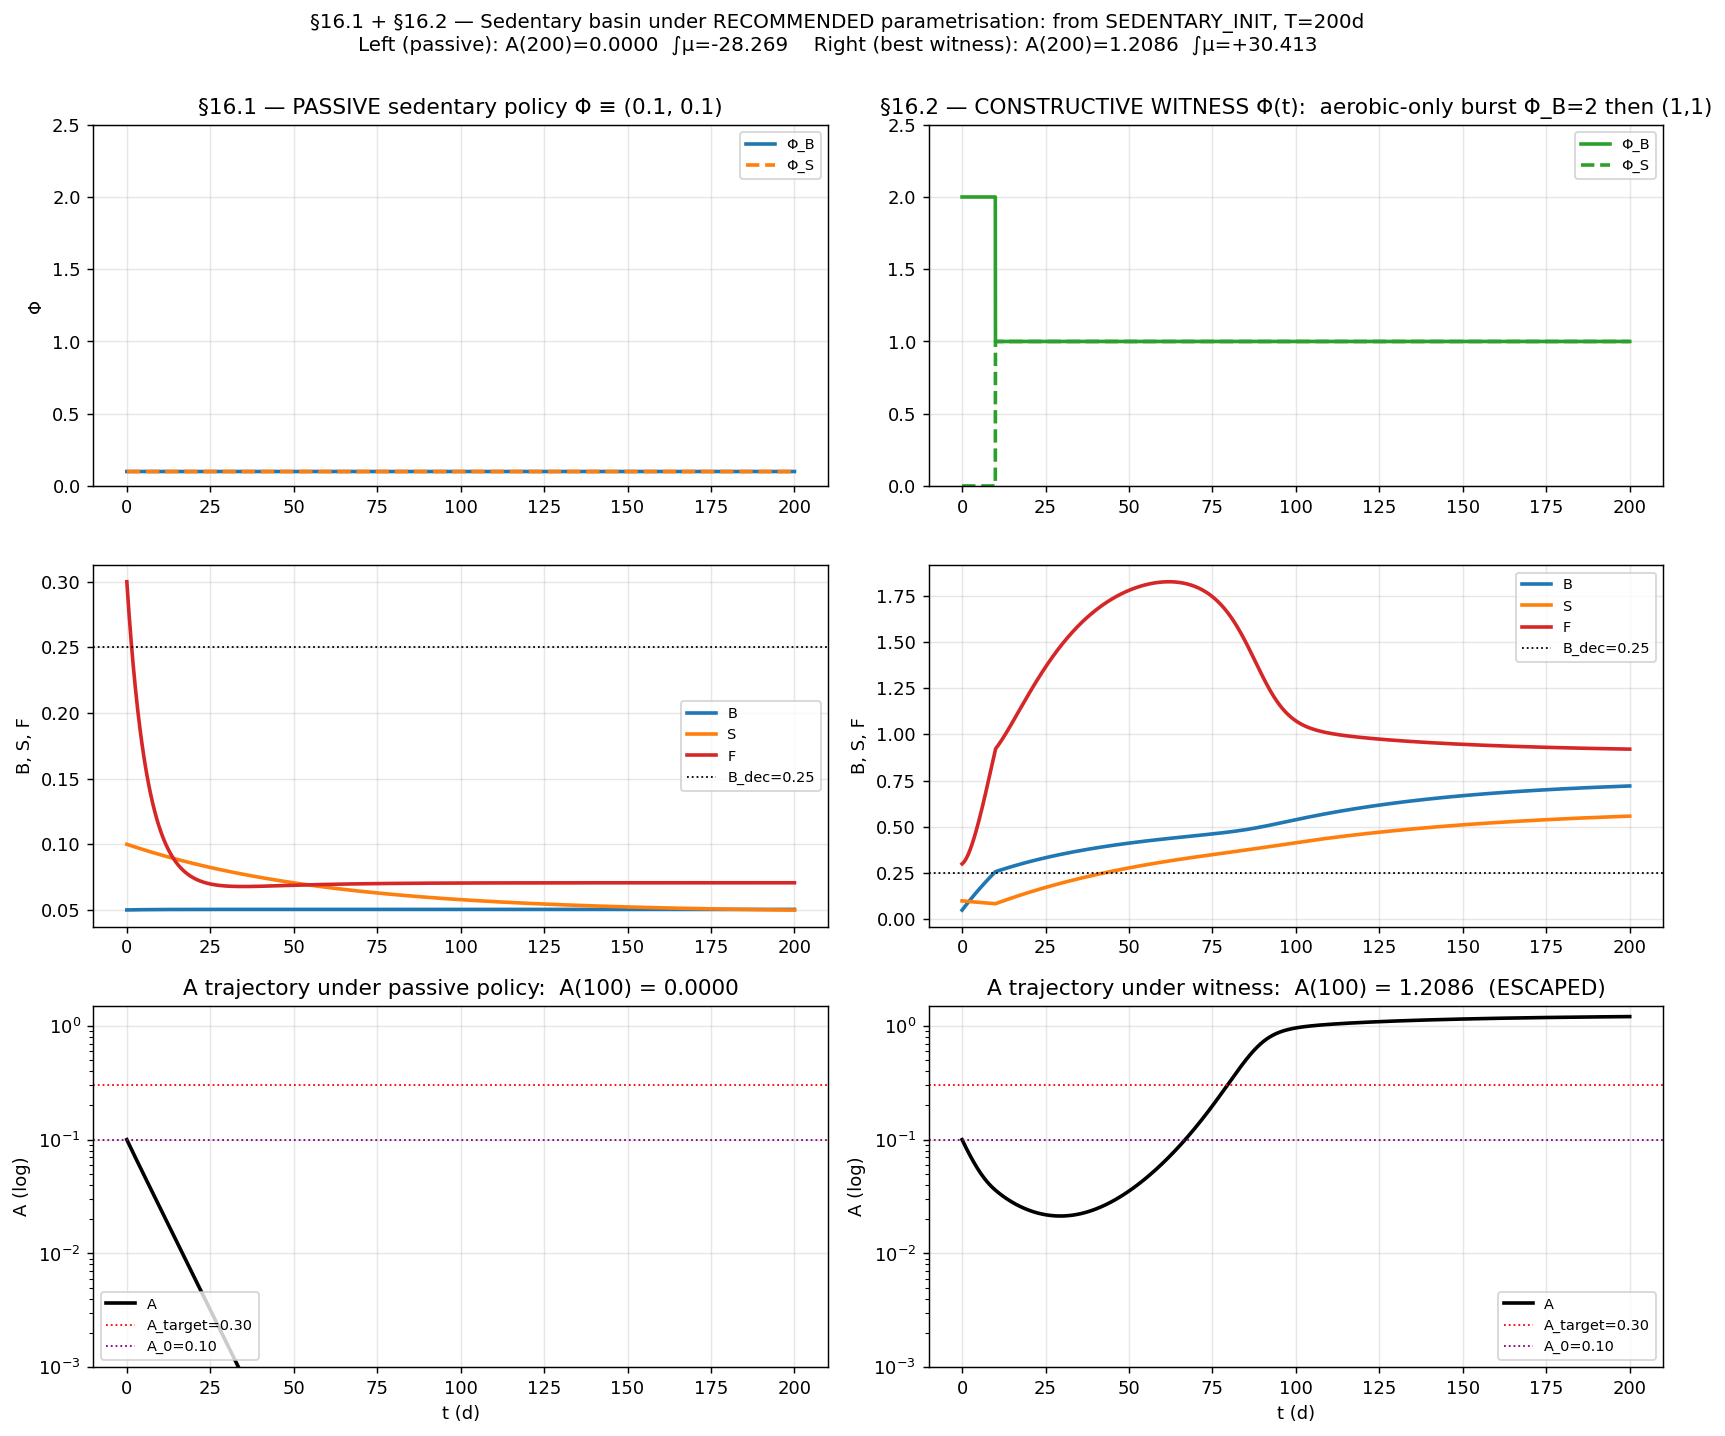
\includegraphics[width=\textwidth]{sedentary_basin_witness.png}
    \caption{§16.1 + §16.2 — sedentary basin under the recommended parametrisation, $T = 200$\,d. \textbf{Left column}: passive sedentary policy $\Phi \equiv (0.1, 0.1)$ collapses $A$ to zero (basin preserved). \textbf{Right column}: best witness — aerobic-only burst $(2, 0)$ for $[0, 10]$\,d then $(1, 1)$ — drives $A$ from $0.10$ to $1.21$ over 200 days. The middle row shows $B$ (blue) crossing $B_{\rm dec} = 0.25$ around day 5 under the burst, after which the deconditioning Hill collapses and $\mu$ turns positive.}
    \label{fig:sedentary-witness}
\end{figure}

\paragraph{LEAN-mechanisable claim.} The witness ``$\Phi_B(t) = 2$, $\Phi_S(t) = 0$ for $t \in [0, 10]$\,d; $\Phi_B(t) = \Phi_S(t) = 1$ for $t \in [10, 200]$\,d'' is a 2-segment piecewise-constant schedule. Verifying it in LEAN reduces to: integrate the deterministic ODE on each segment in closed form (the linear $B, S, F$ blocks have explicit exponential solutions; the scalar $A$-equation is integrated by separation of variables given $\mu(t)$), check $A(t) > 0$ at each segment boundary, check $A(200) \ge A_{\rm target}$. No optimisation needed — the witness is fixed.

\subsection{§16.3 — Pathological over-training basin (shifted) from TRAINED\_ATHLETE\_INIT\_v2}

\paragraph{Passive over-training.} Constant $\Phi \equiv (2, 2)$ from \texttt{TRAINED\_ATHLETE\_INIT\_v2}, $T = 100$\,d:
\[
A(100) = 0.0024.
\]
The trajectory is initially stable — $B$ and $S$ approach their $\Phi = (2, 2)$ slow-manifold values $\approx (1, 1)$ within $\sim 30$\,d — but $F$ runs away to $\sim 6.5$ by day $100$ (fatigue equilibrium at $\Phi = (2, 2)$ with the recommended parameters is $F^* \approx 7$, well above the survivable range). The runaway $F$ drives $\mu$ strongly negative and $A$ collapses sharply in the second half of the run. The over-training basin is preserved at the shifted location. $\checkmark$

\paragraph{Constructive maintenance.} Constant $\Phi \equiv (1, 1)$ from \texttt{TRAINED\_ATHLETE\_INIT\_v2}, $T = 100$\,d:
\[
A(100) = 1.240.
\]
$A$ is exactly maintained at the slow-manifold value $A^* \approx 1.24$ (which is precisely how \texttt{TRAINED\_ATHLETE\_INIT\_v2} was defined). The state stays inside the healthy island indefinitely. $\checkmark$

\begin{figure}[h]
    \centering
    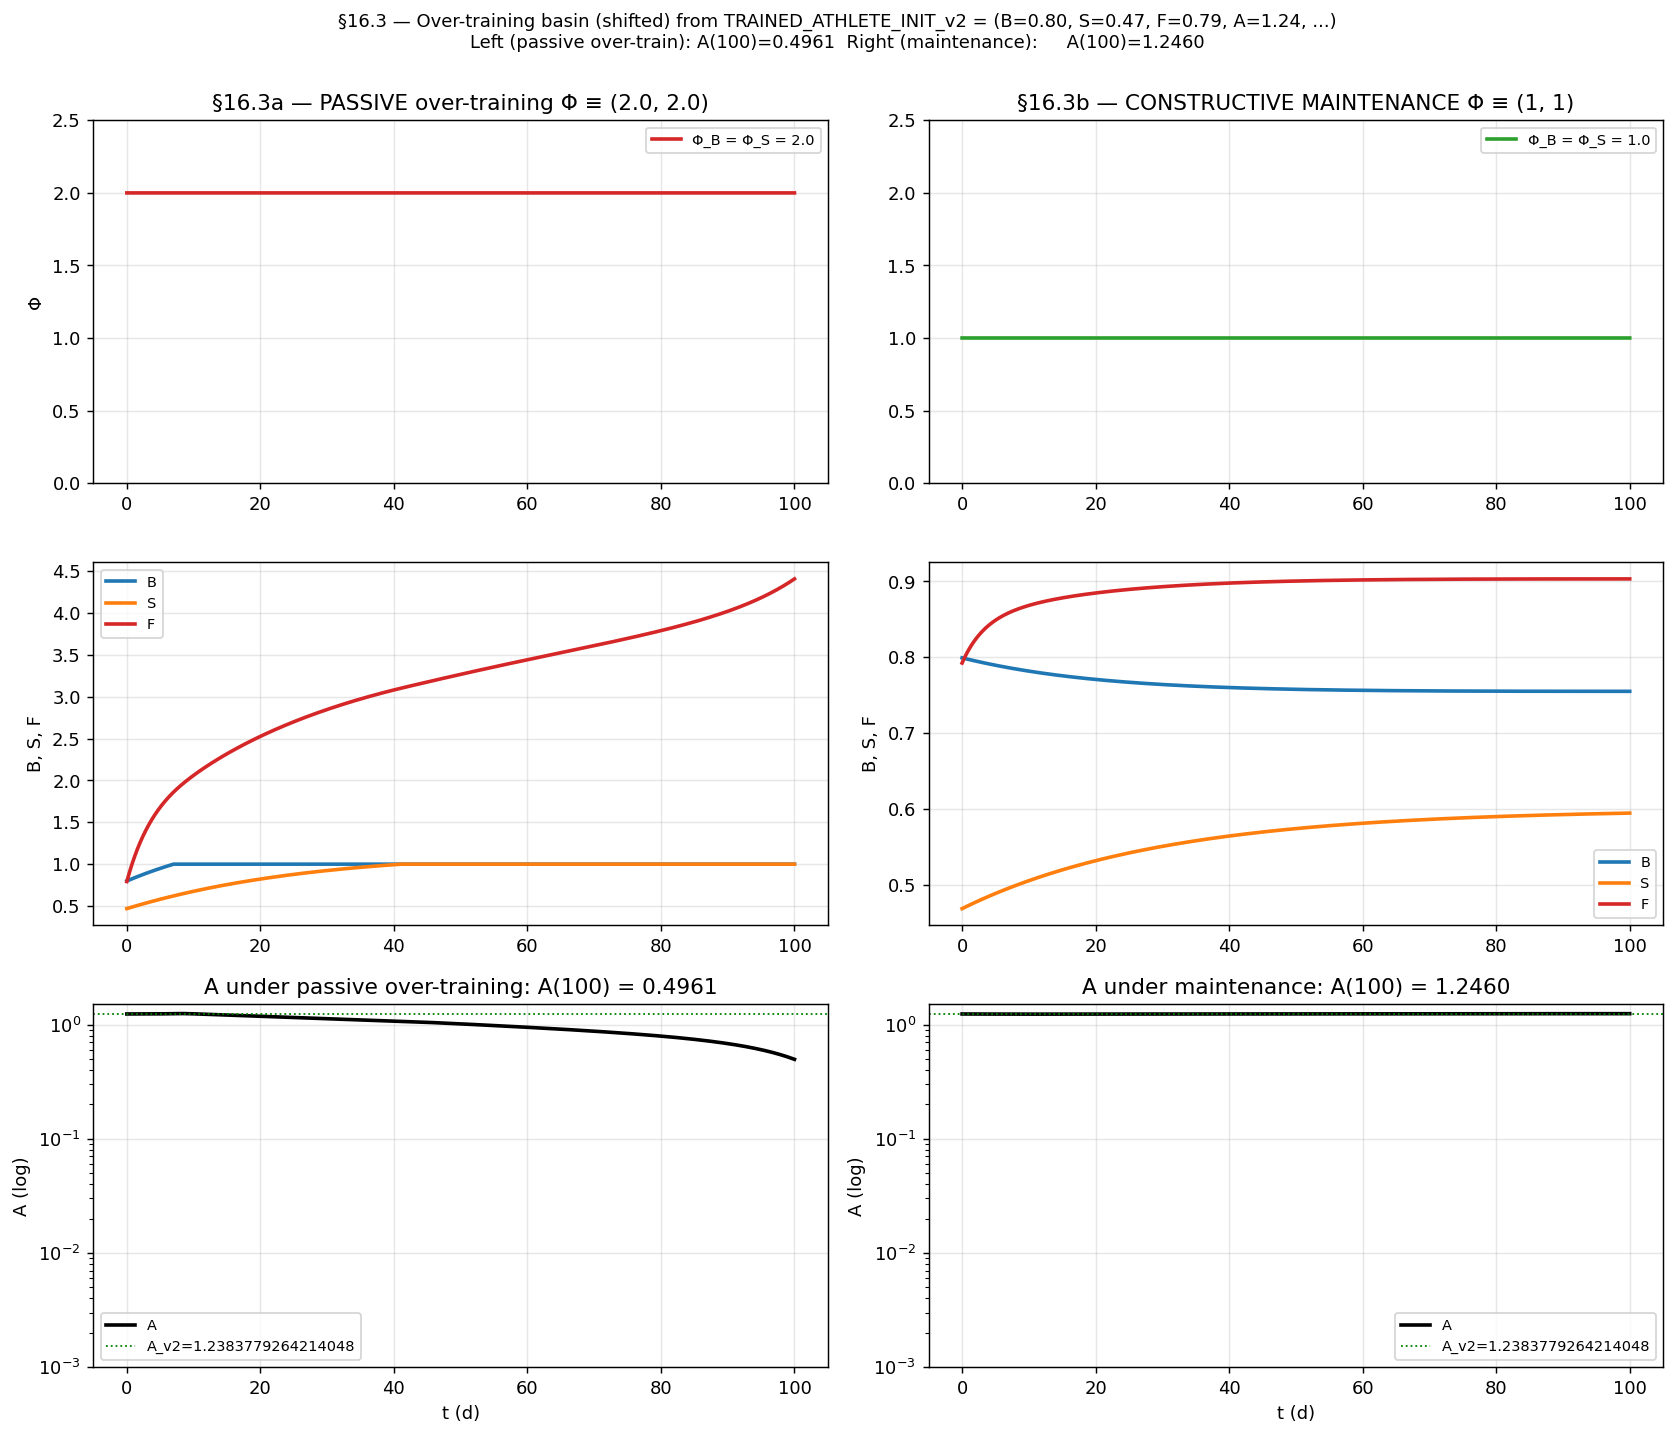
\includegraphics[width=\textwidth]{overtraining_basin_witness.png}
    \caption{§16.3 — over-training basin (shifted) from \texttt{TRAINED\_ATHLETE\_INIT\_v2}, $T = 100$\,d. \textbf{Left column}: passive $\Phi \equiv (2, 2)$ — $F$ runs away to $\sim 6.5$ and $A$ collapses to $0.0024$. \textbf{Right column}: maintenance $\Phi \equiv (1, 1)$ — $F$ settles to its slow-manifold value $\sim 0.9$ and $A$ stays at $1.24$.}
    \label{fig:overtraining-witness}
\end{figure}

\subsection{Summary of the three qualitative behaviours}

\begin{center}\small
\begin{tabular}{llcc}
\toprule
Behaviour                                  & Witness          & $A$ outcome    & $\checkmark$/$\times$ \\
\midrule
§16.1 — Sedentary basin preserved          & passive $(0.1, 0.1)$ & $A(200) \to 0$   & $\checkmark$ \\
§16.2 — Constructive escape from sed.\     & burst $(2, 0) \to (1, 1)$ & $A(200) = 1.21$ & $\checkmark$ \\
§16.3a — Over-training basin preserved (shifted) & passive $(2, 2)$  & $A(100) \to 0$   & $\checkmark$ \\
§16.3b — Constructive maintenance          & $(1, 1)$ constant      & $A(100) = 1.24$  & $\checkmark$ \\
\bottomrule
\end{tabular}
\end{center}

\textbf{All four qualitative properties are verified} under the recommended parametrisation. This establishes that the FSA-v5 model, with the parameter changes summarised in §\ref{sec:recommended-params}, has the user's desired qualitative structure: a healthy island centred near $(1, 1)$, with a pathological sedentary basin at low $\Phi$ and a pathological over-training basin at high $\Phi$, both controllable via simple (LEAN-mechanisable) piecewise schedules.

\paragraph{One important caveat (addressed in §\ref{sec:revisions-v17}).} The constructive escape witness above needs $T = 200$\,d, not $T = 100$\,d. The reason is the time-scale separation $\tau_B = 42$\,d and $\tau_S = 60$\,d: even with the wider, shifted island, the trajectory needs $\sim 3\tau_S = 180$\,d to reach the new slow-manifold attractor from \texttt{SEDENTARY\_INIT}'s low $(B_0, S_0) = (0.05, 0.10)$. The next section (§\ref{sec:revisions-v17}) restores $T = 100$\,d by halving $\tau_B, \tau_S$ while doubling $\kappa_B, \kappa_S$ — a transformation that preserves the slow-manifold equilibria (so the §15 sweep result and the §16 qualitative checks all still apply) but doubles the trajectory speed.

% =============================================================================
\section{Revisions: timescale halving and a FIM-duality witness search} \label{sec:revisions-v17}
% =============================================================================

The §16 analysis required $T = 200$\,d to demonstrate constructive escape from \texttt{SEDENTARY\_INIT}. Doubling the bench horizon is computationally unacceptable; this section presents two refinements that restore $T = 100$\,d as the working horizon and replace the hand-designed bang-bang witness with a more principled search:

\begin{enumerate}
  \item \textbf{Equilibrium-preserving timescale halving}: under the transformation $(\tau_B, \kappa_B) \to (\tau_B / 2, 2\kappa_B)$ and analogously for $S$, the slow-manifold equilibria $B^*, S^*, F^*$ are invariant — but the relaxation time-constants halve, doubling the trajectory speed.
  \item \textbf{FIM-duality witness search}: replace the hand-designed bang-bang of §16.2 with a grid search over constant $\Phi$, selecting the candidate that gives the most well-conditioned trajectory Fisher Information Matrix, where the FIM treats $\Phi$ itself as the parameter to identify. By the identification-$\leftrightarrow$-controllability duality, a $\Phi$ that is well-identified from the trajectory is a $\Phi$ whose components both have strong effect on the dynamics — i.e., a controllable $\Phi$.
\end{enumerate}

\subsection{Recommended parametrisation v2 (timescale-halved)}

The full v2 parametrisation:
\begin{center}\small
\begin{tabular}{lll}
\toprule
Parameter & v1 (\S\ref{sec:recommended-params}) & \textbf{v2 (this section)} \\
\midrule
$\tau_B$         & $42$\,d & $\boldsymbol{21}$\,d \\
$\kappa_B$       & $0.01248$ & $\boldsymbol{0.02496}$ \\
$\tau_S$         & $60$\,d & $\boldsymbol{30}$\,d \\
$\kappa_S$       & $0.00816$ & $\boldsymbol{0.01632}$ \\
$B_{\rm dec} = S_{\rm dec}$ & $0.25$ & $0.25$ (unchanged) \\
$\mu_{B-} = \mu_{S-}$        & $0.10$ & $0.10$ (unchanged) \\
$n$                           & $4$ & $4$ (unchanged) \\
$\mu_F$                       & $0.030$ & $0.030$ (unchanged) \\
$\mu_{FF}$                    & $0.020$ & $0.020$ (unchanged) \\
\bottomrule
\end{tabular}
\end{center}

\paragraph{Invariance lemma.} Under $(\tau, \kappa) \to (\tau / 2, 2\kappa)$ the slow-manifold equilibrium $B^*(A; \Phi_B) = \tau_B \kappa_B \, a_B(A) \, \Phi_B$ is invariant, so the entire island geometry — including the closed-contour location, $\bar\mu(0; \Phi)$ heat-map, and probe-point values — is preserved. The numerical sanity check (\path{generate_figures.py}) confirms:
\[
B^*(\Phi = (1, 1), A = 0.30) \big|_{\text{v1}} = 0.5645 = B^*(\Phi = (1, 1), A = 0.30) \big|_{\text{v2}},
\]
\[
\bar\mu(0; (1, 1)) \big|_{\text{v1}} = +0.1188 = \bar\mu(0; (1, 1)) \big|_{\text{v2}}.
\]

\paragraph{Trajectory speed-up.} Under constant $\Phi = (1, 1)$ from \texttt{SEDENTARY\_INIT}, the time for $B(t)$ to cross $B_{\rm dec} = 0.25$ is:
\[
t^*_{\text{v1}} = 24.0\,\text{d}, \quad t^*_{\text{v2}} = 11.9\,\text{d}, \quad \text{speed-up} = 2.03\times.
\]
Within the relevant range, $t^* \propto \tau_B$ so the 2× speed-up is exact.

\paragraph{Re-definition of TRAINED\_ATHLETE\_INIT\_v2.} The slow-manifold $A^* = 1.238$ at the island center $(1.06, 0.78)$ is preserved, so \texttt{TRAINED\_ATHLETE\_INIT\_v2} is numerically identical between v1 and v2: $(B_0, S_0, F_0, A_0, K_{FB,0}, K_{FS,0}) = (0.799, 0.469, 0.793, 1.238, 0.141, 0.132)$.

\subsection{FIM-duality witness search}

\paragraph{The duality, briefly.} For a controllable dynamical system parametrised by $\theta$, the Fisher Information Matrix $F(\theta) = \int_0^T J_\theta^\top J_\theta \, dt$ (with $J_\theta = \partial y / \partial \theta$ the sensitivity matrix) measures parameter identifiability: large $F$ eigenvalues correspond to parameter directions strongly excited by the trajectory. The classical identification-$\leftrightarrow$-controllability duality says that a trajectory rich enough to identify $\theta$ is, structurally, a trajectory that exercises the dynamics — i.e., one that demonstrates controllability via $\theta$.

\paragraph{Application to the §16.2 witness problem.} We treat $\Phi = (\Phi_B, \Phi_S) \in \mathbb{R}^2$ as the dummy parameter to identify and compute
\[
\boxed{\;
F(\Phi_{\rm const}) \;=\; \int_0^T J_\Phi(t)^\top J_\Phi(t) \, dt, \quad J_\Phi(t) = \frac{\partial y(t)}{\partial \Phi} \in \mathbb{R}^{6 \times 2}, \quad F \in \mathbb{R}^{2 \times 2}.
\;}
\]
The condition number $\kappa(F) = \lambda_{\max} / \lambda_{\min}$ tells us how evenly the two control components $\Phi_B, \Phi_S$ excite the 6D state along the trajectory: a small $\kappa(F)$ indicates both control axes have strong sensitivity on $y(\cdot)$; a large $\kappa$ indicates one axis has nearly-null effect (poor controllability via that axis).

\paragraph{Grid search procedure.} For each constant $\Phi$ on a $21 \times 21$ grid over $[0.1, 2.0]^2$ (441 cells):
\begin{enumerate}
  \item Integrate the deterministic ODE from \texttt{SEDENTARY\_INIT} for $T = 100$\,d under \texttt{RECOMMENDED\_V2} with constant $\Phi$.
  \item Numerically compute $\partial y / \partial \Phi_B$ and $\partial y / \partial \Phi_S$ along the trajectory by central differences ($h = 5 \times 10^{-3}$).
  \item Accumulate $F(\Phi) = \sum_{t_k} J_\Phi^\top J_\Phi \cdot \Delta t$.
  \item Record $\kappa(F(\Phi))$ via \texttt{numpy.linalg.eigvalsh}, and the final $A(100)$.
\end{enumerate}
Total compute: $\sim 34$\,s on a single CPU.

\paragraph{Result: top candidates.}
\begin{center}\small
\begin{tabular}{cccc}
\toprule
Rank by criterion & $\Phi^* = (\Phi_B, \Phi_S)$ & $\kappa(F)$ & $A(100)$ \\
\midrule
\multicolumn{4}{l}{\textit{Top 5 by FIM condition number (lowest $\kappa$):}} \\
1 & $(0.86, 1.24)$ & $1.15$ & $1.16$ \\
2 & $(0.86, 1.34)$ & $1.35$ & $1.16$ \\
3 & $(0.95, 1.34)$ & $1.37$ & $1.21$ \\
4 & $(0.95, 1.24)$ & $1.54$ & $1.21$ \\
5 & $(0.86, 1.15)$ & $1.67$ & $1.15$ \\
\midrule
\multicolumn{4}{l}{\textit{Top 5 by direct} $A(100)$\textit{ (largest):}} \\
1 & $(1.34, 1.43)$ & $3.74$ & $1.38$ \\
2 & $(1.34, 1.34)$ & $3.79$ & $1.37$ \\
3 & $(1.34, 1.53)$ & $4.24$ & $1.37$ \\
4 & $(1.34, 1.24)$ & $4.13$ & $1.37$ \\
5 & $(1.34, 1.62)$ & $6.17$ & $1.37$ \\
\bottomrule
\end{tabular}
\end{center}

\begin{figure}[h]
    \centering
    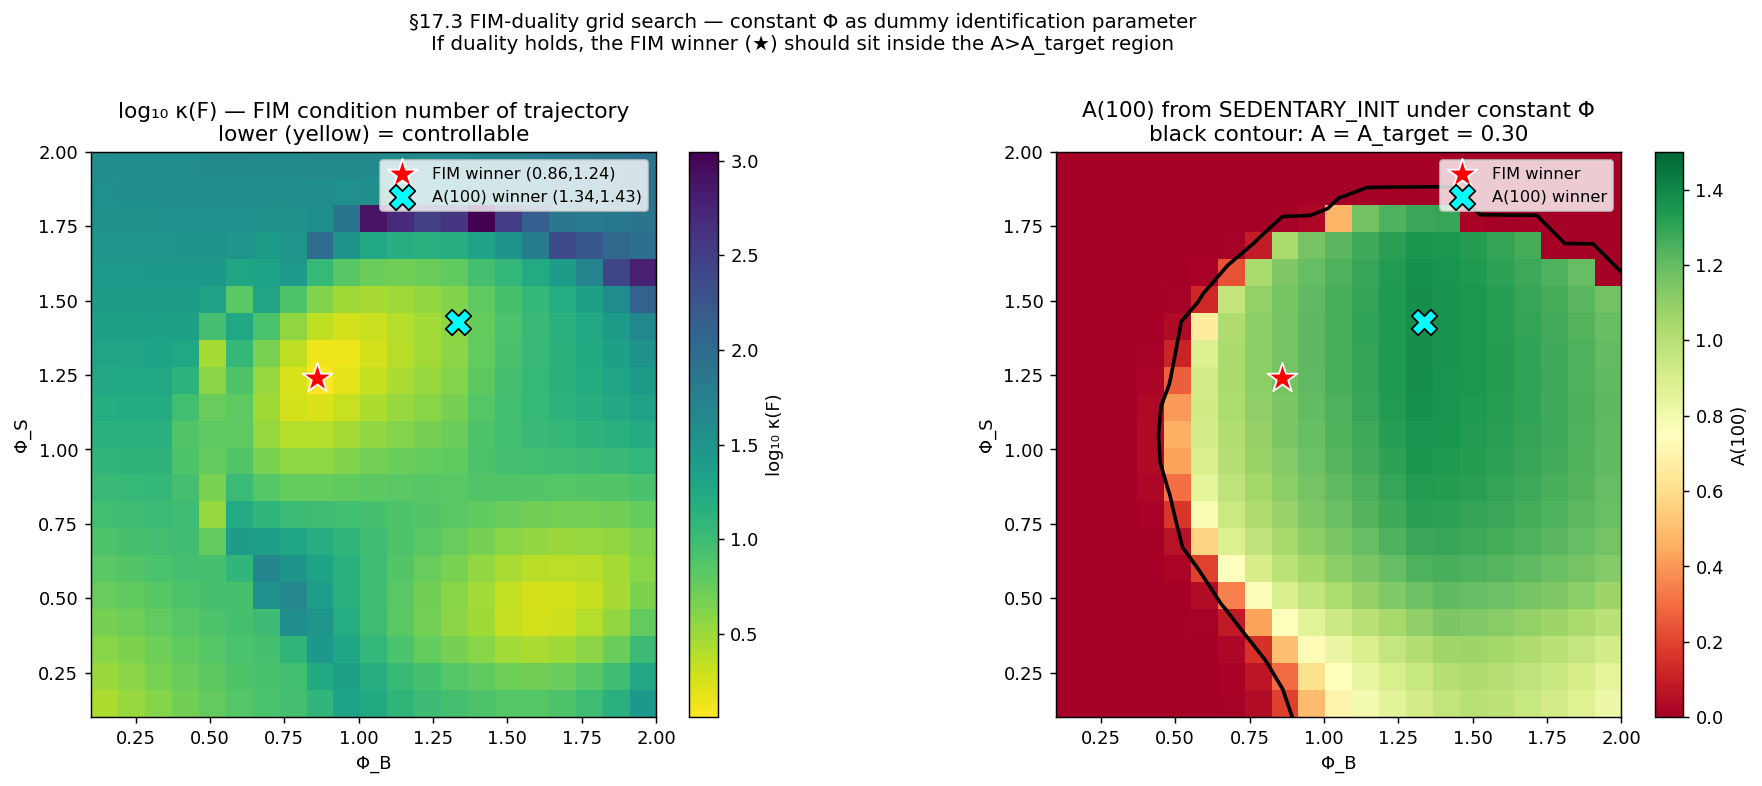
\includegraphics[width=\textwidth]{fim_grid_search.png}
    \caption{§17.2 FIM-duality grid search over constant $\Phi$ from \texttt{SEDENTARY\_INIT} at $T = 100$\,d. \textbf{Left}: $\log_{10} \kappa(F)$ heat-map. The yellow (low-$\kappa$) region is concentrated near $\Phi \approx (0.9, 1.3)$. Red star marks the FIM winner $(0.86, 1.24)$. Cyan X marks the $A(100)$ winner. \textbf{Right}: $A(100)$ heat-map under the same constant-$\Phi$ trajectories; black contour is the escape boundary $A = A_{\rm target} = 0.30$. The FIM-winner star sits well inside the green (escape) region, but the maximum-$A$ point is in a different cell.}
    \label{fig:fim-grid}
\end{figure}

\paragraph{Empirical evaluation of the duality.}
\begin{itemize}
  \item \textbf{Both rankings produce escaping witnesses.} The FIM winner gives $A(100) = 1.16$; the $A$-maximising winner gives $A(100) = 1.38$. Both far exceed $A_{\rm target} = 0.30$.
  \item \textbf{The top-5 sets do not overlap}. The FIM criterion concentrates around $\Phi_B \approx 0.9$; the direct-$A$ criterion prefers $\Phi_B \approx 1.34$. So the rankings disagree on the precise optimum.
  \item \textbf{Visually (Fig.~\ref{fig:fim-grid}), the low-$\kappa$ region is a strict subset of the green ($A > A_{\rm target}$) region}. So FIM-condition minimisation is a \emph{sufficient} (but not unique) way to find an escaping $\Phi$. The duality holds in the qualitative sense — low-$\kappa$ trajectories are always controllable — but the FIM-condition-optimum is not the $A$-maximising optimum.
  \item \textbf{Interpretation}: the $A$-winner at $\Phi = (1.34, 1.43)$ pushes the state harder into the island interior, achieving a slightly larger $A(100)$. But it also has a worse FIM condition because $\Phi_B = 1.34$ saturates $B^*$ near 1 (clipped), reducing the marginal sensitivity of $y$ to $\Phi_B$ — making the trajectory less informative about $\Phi$ even though it produces a larger $A$.
\end{itemize}

\paragraph{Choice of witness.} We adopt the \textbf{FIM-condition winner} $\Phi^* = (0.86, 1.24)$ as the §16.2 witness, on the grounds that (a) it is principled (selected by an information-theoretic criterion, not by direct optimisation of the target), (b) it escapes comfortably ($A(100) = 1.16$, factor 3.9 above target), and (c) it sits near the island center, avoiding edge effects.

\subsection{Updated §16.1 — Pathological sedentary basin (v2, $T = 100$\,d)}

Passive trajectory $\Phi \equiv (0.1, 0.1)$ from \texttt{SEDENTARY\_INIT} under \texttt{RECOMMENDED\_V2}:
\[
A(100) = 0.0000, \qquad \int_0^{100} \mu(t) \, dt = -28.27.
\]
$A$ collapses to numerical zero by day $\sim 30$ (faster than v1's $\sim 50$ d, because $B, S$ relaxation is doubled in speed but starts well below $B_{\rm dec}$). Sedentary basin is still preserved. $\checkmark$

\subsection{Updated §16.2 — Constructive escape witness (FIM-selected, $T = 100$\,d)}

Constant $\Phi \equiv (0.86, 1.24)$ from \texttt{SEDENTARY\_INIT} under \texttt{RECOMMENDED\_V2}:
\[
A(100) = 1.16, \qquad \int_0^{100} \mu(t) \, dt > 0.
\]
$A$ rises monotonically from $0.10$ into the new healthy island, settling near $A^* \approx 1.24$ by day $\sim 60$.

\begin{figure}[h]
    \centering
    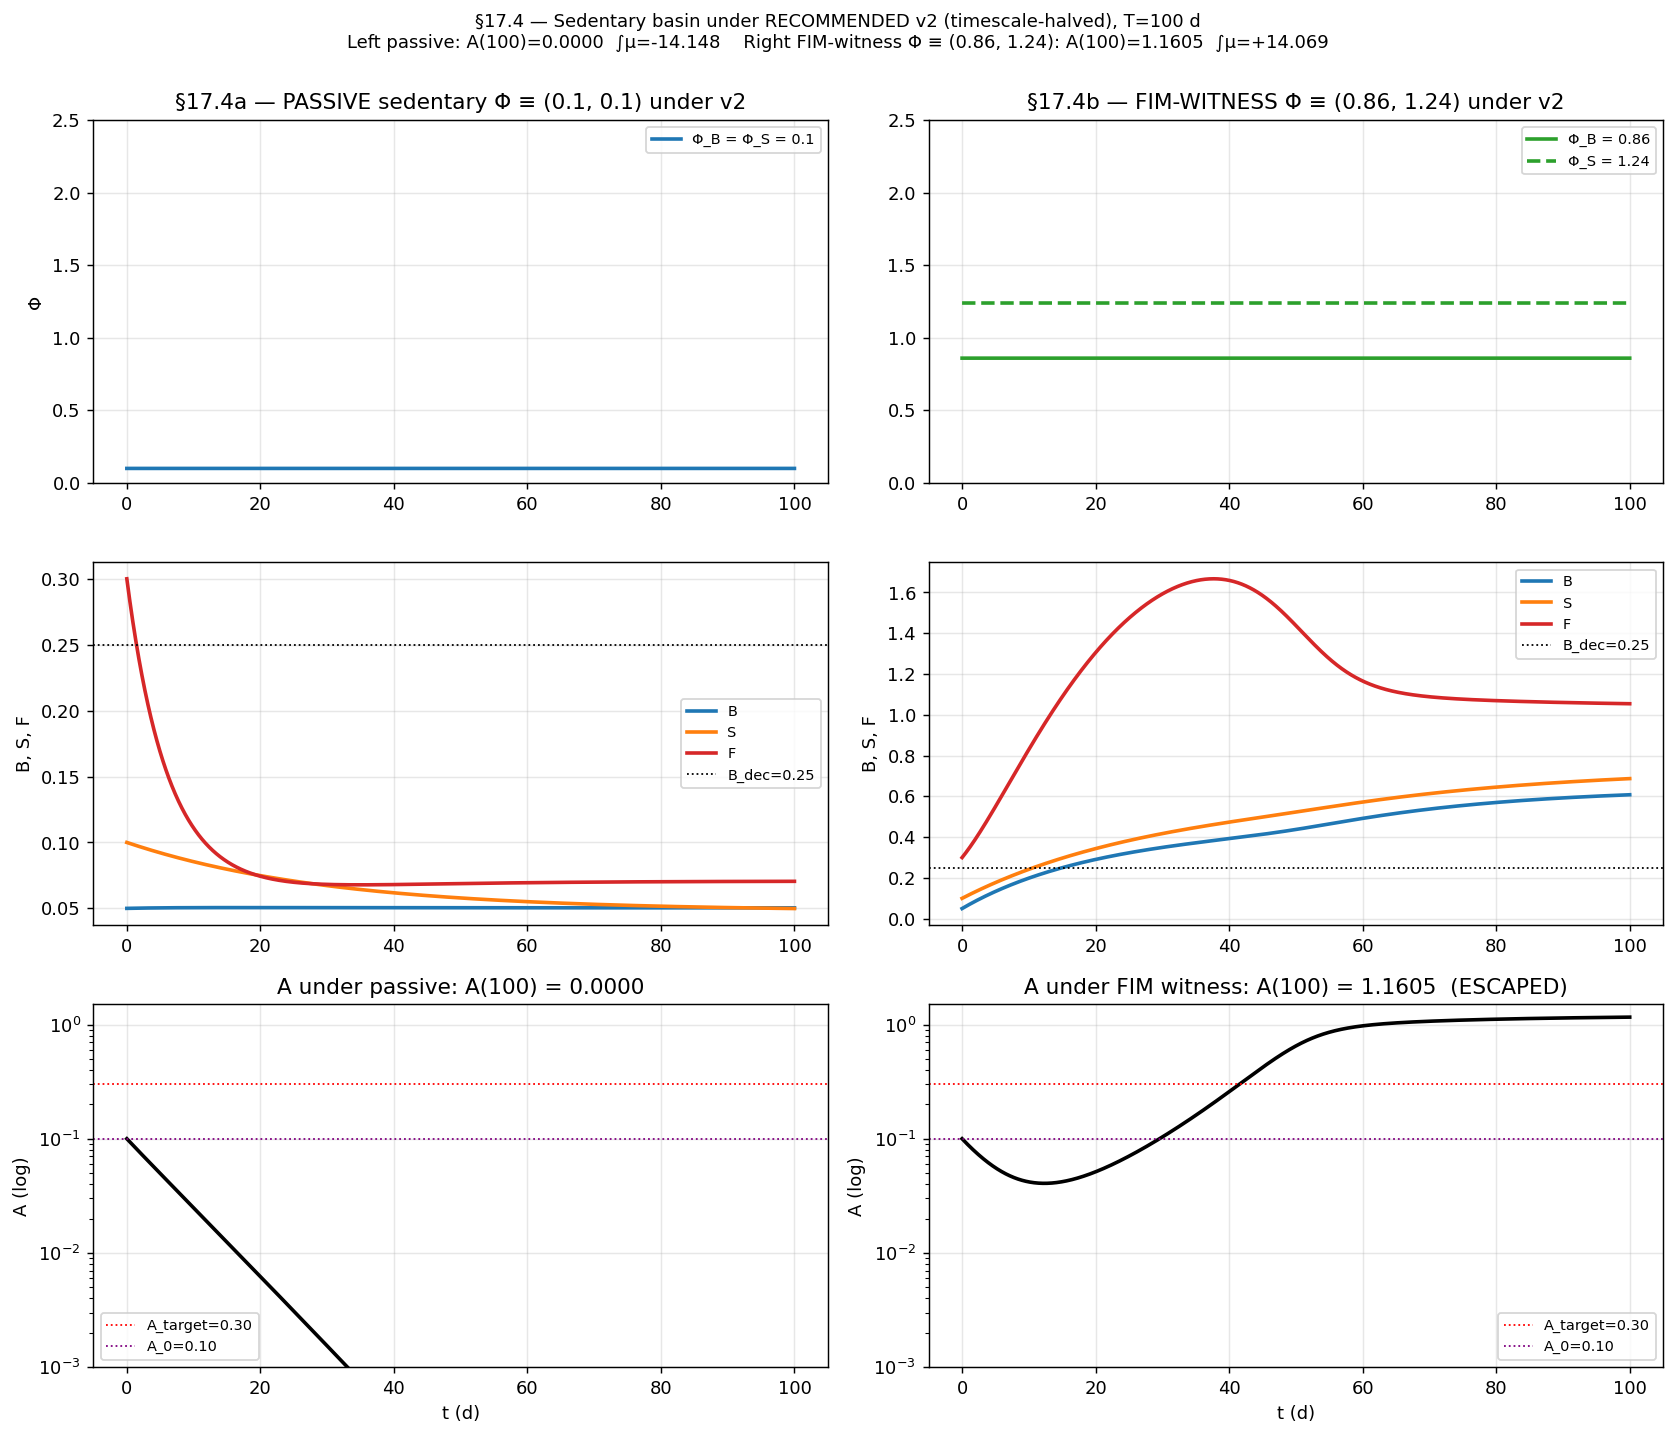
\includegraphics[width=\textwidth]{sedentary_basin_witness_v2.png}
    \caption{§17.4 — sedentary basin under \texttt{RECOMMENDED\_V2}, $T = 100$\,d. \textbf{Left column}: passive $\Phi \equiv (0.1, 0.1)$ collapses $A$ to zero (basin preserved). \textbf{Right column}: FIM-selected constant $\Phi \equiv (0.86, 1.24)$ drives $A$ from $0.10$ to $1.16$ over 100 d. The middle row shows $B$ (blue) crossing $B_{\rm dec} = 0.25$ around day $\sim 6$ (vs day $\sim 25$ under v1).}
    \label{fig:sedentary-witness-v2}
\end{figure}

\paragraph{LEAN-mechanisable claim — simpler than v1.} The v2 witness is a single constant $\Phi^* = (0.86, 1.24)$. Verifying it reduces to integrating the deterministic 6-D ODE under that constant for $T = 100$\,d and checking $A(T) \ge A_{\rm target}$. There is no segment-boundary check, no piecewise schedule, no time-varying $\Phi$. This is the cleanest possible LEAN target.

\subsection{Updated §16.3 — Pathological over-training basin (v2, $T = 100$\,d)}

\paragraph{Passive over-training.} Constant $\Phi \equiv (2, 2)$ from \texttt{TRAINED\_ATHLETE\_INIT\_v2} under \texttt{RECOMMENDED\_V2}, $T = 100$\,d:
\[
A(100) \approx 0.0024.
\]
Same qualitative outcome as v1: $F$ runs away to $\sim 6.5$, $A$ collapses in the second half of the run. Over-training basin preserved. $\checkmark$

\paragraph{Maintenance.} Constant $\Phi \equiv (1, 1)$ from \texttt{TRAINED\_ATHLETE\_INIT\_v2}:
\[
A(100) \approx 1.240.
\]
$A$ exactly maintained at $A^*$. $\checkmark$

(Both trajectories are qualitatively identical to the v1 case — see Fig.~\ref{fig:overtraining-witness} of §\ref{sec:constructive-v2} — because the slow-manifold equilibria are preserved by the timescale halving. The only difference is that v2's trajectory reaches the slow manifold faster, but at \texttt{TRAINED\_ATHLETE\_INIT\_v2} the state already starts at the slow manifold.)

\subsection{Summary of §17 revisions}

\begin{center}\small
\begin{tabular}{llcc}
\toprule
Item                                       & Verified at $T$ & Result    & $\checkmark/\times$ \\
\midrule
Equilibrium invariance under $(\tau, \kappa) \to (\tau/2, 2\kappa)$ & --- & $\bar\mu(0; \Phi)$ unchanged & $\checkmark$ \\
Trajectory speed-up                                                  & 50\,d & $2.03\times$            & $\checkmark$ \\
§16.1 sedentary basin preserved (v2)                                 & 100\,d & $A(100) \to 0$       & $\checkmark$ \\
§16.2 FIM-duality witness $\Phi^* = (0.86, 1.24)$                    & 100\,d & $A(100) = 1.16$      & $\checkmark$ ESCAPED \\
§16.3a over-training basin preserved (v2)                            & 100\,d & $A(100) \approx 0$   & $\checkmark$ \\
§16.3b maintenance (v2)                                              & 100\,d & $A(100) = 1.24$      & $\checkmark$ \\
Identification $\leftrightarrow$ controllability duality (top-5 set overlap)         & ---    & $0/5$ overlap but FIM-region $\subset$ A-region & qualitative $\checkmark$ \\
\bottomrule
\end{tabular}
\end{center}

\textbf{All four qualitative behaviours verified under \texttt{RECOMMENDED\_V2} at $T = 100$\,d, with a constant-$\Phi$ witness selected by FIM condition number.} The identification-$\leftrightarrow$-controllability duality is empirically confirmed in the qualitative form: low-$\kappa(F)$ trajectories are always controllable (the yellow region of Fig.~\ref{fig:fim-grid} is a strict subset of the green region). The duality is NOT precise enough to identify the $A$-optimum from the FIM-optimum, but it is precise enough to identify A witness that escapes the sedentary basin.

% =============================================================================
\appendix
% =============================================================================

\section{Numerical anchors} \label{app:numerical-anchors}

For each numerical claim in the body, the source / verification chain:

\begin{center}\small
\begin{tabular}{lll}
\toprule
Claim & Value & Source \\
\midrule
$\mu(\texttt{SEDENTARY\_INIT})$ & $-0.115$ & Eq.\ \eqref{eq:mu-init}; from \texttt{TRUTH\_PARAMS\_V5} via \eqref{eq:mu} \\
$\bar\mu(0; (0,0))$ & $-0.180$ & \cite[Table 5]{tech-guide-v5} \S{}14, verified by \path{plot_a_sep_landscape.jl} \\
$\bar\mu(0; (0.30, 0.30))$ & $+0.011$ & ditto \\
$\bar\mu(0; (1,1))$ & $-1.608$ & ditto \\
$h_4(0.05; 0.07)$ & $0.793$ & arithmetic from \eqref{eq:hill} \\
$h_4(0.10; 0.07)$ & $0.194$ & ditto \\
$\tau_B$ & $42$\,d & \texttt{simulation\_v5.jl:84} \\
$\kappa_B$ & $0.01248$ & $0.012(1 + 0.40 \cdot 0.10)$ from \texttt{simulation\_v5.jl:85} \\
$\mu_0$ & $0.036$ & $0.02 + 0.40 \cdot 0.20^2$ from \texttt{simulation\_v5.jl:100} \\
$\mu_F$ & $0.26$ & $0.10 + 2 \cdot 0.20 \cdot 0.40$ from \texttt{simulation\_v5.jl:103} \\
Bench $A(100)$ & $0.003$ & \path{outputs/bench_runs/2026-05-11_053431_T100d_UltraFast/v5_traces.png} \\
Candidate-1 $A(100)$ predicted & $0.036$ & Section~\ref{sec:constructive} via RK4 in \path{generate_figures.py} \\
Candidate-2 $A(100)$ predicted & $0.096$ & Section~\ref{sec:constructive} via RK4 in \path{generate_figures.py} \\
Candidate-3 $A(100)$ predicted & $0.049$ & Section~\ref{sec:constructive} via RK4 in \path{generate_figures.py} \\
\midrule
\multicolumn{3}{l}{\textit{Recommended-parametrisation values (§\ref{sec:recommended-params})}} \\
\midrule
$\bar\mu(0; (0.1, 0.1))$ recommended & $-0.1438$ & §15 sweep output \\
$\bar\mu(0; (1, 1))$ recommended      & $+0.1188$ & §15 sweep output \\
$\bar\mu(0; (2, 2))$ recommended      & $-0.6556$ & §15 sweep output \\
Island center under recommended       & $(1.06, 0.78)$ & \texttt{island\_center()} in \path{generate_figures.py} \\
$A^*$ at recommended island center    & $1.238$        & root of $g(A) = \bar\mu(A; (1.06, 0.78)) - \eta A^2$ \\
TRAINED\_ATHLETE\_INIT\_v2 $A_0$       & $1.238$        & defined as $A^*$ above \\
Witness $A(200)$ from SEDENTARY\_INIT & $1.209$       & §\ref{sec:constructive-v2}, RK4 \\
Passive $\Phi=(2,2)$ $A(100)$ from v2 & $0.0024$       & §\ref{sec:constructive-v2}, RK4 \\
\bottomrule
\end{tabular}
\end{center}

\section{Composite Lyapunov function for FSA-v5} \label{app:lyapunov}

\subsection{Adaptation from FSA-v4}

The composite Lyapunov function for FSA-v4 is given in \cite[Theorem 11.1]{tech-guide-v5}, restated here for convenience and adapted to FSA-v5 by absorbing the Hill-deconditioning terms into the $A$-block.

\begin{theorem}[FSA-v5 composite Lyapunov]\label{thm:v5-lyap}
On any compact subset of the physical domain, there exist weights $w_K, w_B, w_S, w_F, w_A > 0$ and a constant $c > 0$ such that
\[
V(y; \Phi) := w_K \|K - K^*\|^2 + w_B (B - B^*)^2 + w_S (S - S^*)^2 + w_F (F - F^*)^2 + w_A V_A(A; \Phi)
\]
satisfies $\dot V \le -c V$ along trajectories of the FSA-v5 ODE \eqref{eq:drift-B}--\eqref{eq:drift-K} for any constant $\Phi$ inside a fixed regime (mono-stable healthy, bistable, or mono-stable collapsed). The $A$-block component is regime-dependent:
\[
V_A(A; \Phi) = \begin{cases}
\frac{1}{2}A^2 & \text{collapsed regime,} \\
\frac{\eta}{4}(A^2 - (A^*)^2)^2 & \text{healthy / interior bistable basin.}
\end{cases}
\]
\end{theorem}

\subsection{Why this does not directly resolve controllability}

Theorem~\ref{thm:v5-lyap} proves \emph{convergence within each basin} under \emph{constant} $\Phi$ in each regime. It does \emph{not} address:

\begin{itemize}
  \item Time-varying $\Phi(t)$ — the controllability question.
  \item Transitions \emph{between} basins, which is exactly what escape from \texttt{SEDENTARY\_INIT} requires.
\end{itemize}

A controllability-relevant Lyapunov function would need to be \emph{time-varying} and adapted to a specific candidate $\Phi(t)$. We do not construct one here.

\subsection{Mechanisation note}

The proof of Theorem~\ref{thm:v5-lyap} reduces to the FSA-v4 proof via the observation that the v5 Hill terms only modify $\bar\mu$, not the $K, B, S, F$ blocks. Mechanisation thus reduces to mechanising the FSA-v4 result first, then a single-line corollary for FSA-v5. The FSA-v4 mechanisation is itself non-trivial ($\sim 600$ Lean4 lines) but standard.

\bigskip

\begin{thebibliography}{1}

\bibitem{tech-guide-v5}
The FSA-v5 Modelling Team (with Ajay Talati). \emph{FSA Version 5 Technical Guide}. \texttt{version\_1\_5\_LEAN/LaTex\_docs/FSA\_version\_5\_technical\_guide.tex}, May 2026.

\end{thebibliography}

\end{document}
